%%This is a very basic article template.
%%There is just one section and two subsections.

\documentclass[12pt,oneside]{book}
\usepackage{apacite}
\newcommand{\HRule}{\rule{\linewidth}{0.5mm}}

\usepackage[pdftex]{graphicx}
\usepackage{color}
\usepackage{setspace}
\usepackage{fancyhdr}
\usepackage[spanish]{babel}
%\renewcommand\spanishtablename{Tabla}
\usepackage{amssymb}
\usepackage[letterpaper]{geometry}
\usepackage{lscape}
\usepackage{indentfirst}
\usepackage[pdffitwindow]{hyperref}
\usepackage{array}
\usepackage{booktabs}
\hypersetup{
    colorlinks,%
    citecolor=black,%
    filecolor=black,%
    linkcolor=black,%
    urlcolor=black
}
\usepackage[toc]{glossaries}
\usepackage{float}

\raggedbottom

% Use input characters instead of escape codes


\usepackage{titlesec}
\titlespacing{\chapter}{0pt}{-40pt}{10pt}
\titleformat{\chapter}[hang]{\normalfont\huge\bfseries}{\chaptertitlename\
\thechapter}{20pt}{\Huge}
\selectlanguage{spanish}

%\usepackage[apaciteclassic]{apacite}
\usepackage       {apacite}                                                          
%bibliography in apa-style
\usepackage{tocbibind}
\usepackage{textcomp} 
\usepackage{fancybox}% http://ctan.org/pkg/fancybox
\usepackage{lipsum}% http://ctan.org/pkg/fancybox
\makeglossaries
% We define some strings that will use along
\def\thesistitle{Dise\~{n}o de un modelo de red neuronal para un sistema de
control de tr\'{a}nsito distribuido, utilizando el modelo de propagaci\'{o}n
hacia atr\'{a}s para su entrenamiento.}


\begin{document}
\frontmatter
\pagestyle{empty}

\begin{titlepage}
	\begin{center}
		
\includegraphics[scale=0.5]{images/logoUNA.png}
	\end{center}
	\begin{center}	
	\definecolor{unablue}{rgb}{0.016,0.173,0.322}
	\textcolor{unablue}{%
		\textsc{\LARGE Escuela de Inform\'{a}tica}
		\\[0.2cm]
		\textsc{\large Programa de Licenciatura en Sistemas de
		Informaci\'{o}n}
		\\
	}
	\vfill
	 
	% Title
		
		% Title
	\HRule 
	\\[0.9cm]
	\doublespacing
	{
		\large
		\bfseries
		\thesistitle
	}
	\\[0.4cm]
	\singlespacing
	\HRule 
	\\[1.4cm]

	{
		\large Tesis para optar por el grado de 
		\\[0.6cm]
		Licenciatura con \'{E}nfasis en Sistemas de
		Informaci\'{o}n
	}
	\\
	\vfill
	 
	% Author and supervisor
	\begin{minipage}{0.45\textwidth}
		\begin{flushleft} 
			\large
			\textsc{Tesiario:}\\
			{Mag Yari Guevara Rivera}
		\end{flushleft}
	\end{minipage}
	\begin{minipage}{0.50\textwidth}
		\begin{flushright} 
			\large
			\textsc{Director de Tesis:}\\
			{Msc. Eddy Ram\'{i}rez Jim\'{e}nez}
		\end{flushright}
	\end{minipage}

	\vfill
	
	% Bottom of the page
	{
		\large Fecha: Marzo 2012
	}
	\end{center}
\end{titlepage}
\textbf{\LARGE{Presentaci\'{o}n}}\\\\

\textbf{Nombre de la tesis}


Dise\~{n}o de un modelo de red neuronal para un sistema de control de
tr\'{a}nsito distribuido, utilizando el modelo de propagaci\'{o}n hacia atr\'{a}s para su entrenamiento.\\

\textbf{Modalidad}

Tesis. \\
	
\textbf{Encargado}

Mag Yari Guevara Rivera \\
	
\textbf{Nombre del tutor}


 Msc. Eddy Ram\'{i}rez Jim\'{e}nez \\
	 
	
\textbf{Duraci\'{o}n}

 I Ciclo 2012, II Ciclo 2012 y I Ciclo 2013
\tableofcontents
\listoffigures
\listoftables

\mainmatter
% Use double space 
\onehalfspace 
% Now fancy style
\pagestyle{fancy}
% Left the right header clean
\rhead{}
	
%\chapter*{Introducci\'{o}n}
\chapter*{Introducci\'{o}n}\addcontentsline{toc}{chapter}{Introducci\'{o}n}
	\label{chap:introduction}
  
	%\section*{Introducci\'{o}n}

		 
		La incorporaci\'{o}n de nuevos veh\'{i}culos a la flota vehicular con la que cuenta
	actualmente el pa\'{i}s, ha causado un incremento en los tiempos requeridos para
	poder desplazarse en \'{a}reas altamente transitadas, como es el caso de la Gran
	\'{A}rea Metropolitana (GAM). Por otro lado, este problema trae consigo un aumento
	en la emisi\'{o}n de gases contaminantes. Seg\'{u}n estudios del Dr. Dobles
	\cite{Robles2011} , en Costa Rica, la principal fuente de emisi\'{o}n de gases que contribuyen con el efecto invernadero es el consumo de energ\'{i}a en el sector de transporte que consume combustibles importados derivados del petr\'{o}leo, que finalmente terminan afectando al medio ambiente y sobre todo a las personas que se encuentra dentro o en los alrededores de estas \'{a}reas v\'{i}ctimas de este congestionamiento.
	
		Frente a este tipo de eventos, en diferentes pa\'{i}ses se han implementado
	sistemas de control de tr\'{a}fico, los cuales incluyen una red de sem\'{a}foros que
	pueden ser controlados de forma remota desde un centro de control. La ciudad de
	New York fue una de las primeras en implementar un sistema de este tipo
	\cite{Greenman1998}, con un solo edificio localizado en Queens en las oficinas
	del Centro de Control de Tr\'{a}fico perteneciente al Departamento de tr\'{a}nsito.
	
		La idea de estos sistemas, es contar con c\'{a}maras o alg\'{u}n tipo de sensor que le
	permita a un operador, o al mismo sem\'{a}foro, obtener la informaci\'{o}n necesaria
	para poder tomar una decisi\'{o}n, as\'{i} como el registro de la misma para futuras
	labores que se vean afectadas por \'{e}stos.
	
		El lograr que los sem\'{a}foros tomen decisiones \textit{inteligentes}, se ha
	intentado lograr de diferentes formas con soluciones por medio de  algoritmos basados en Inteligencia
	artificial. Rajendra en su libro, describe como el objetivo de la
	Inteligencia Artificial (AI de sus siglas en ingl\'{e}s), es tratar de lograr que
	las computadoras de alguna forma realicen las labores en la que los humanos son
	buenos. La definici\'{o}n de inteligencia artificial tiende a variar entre los
	autores, no obstante Rajendra hace menci\'{o}n de una que deja bastante claro su significado:

		\begin{quote}
			\textit{``Inteligencia artificial es la parte de las ciencias de
			la computaci\'{o}n interesada en dise\~{n}ar sistemas de computaci\'{o}n inteligentes que exhiban las
			caracter\'{i}sticas que se asocian con la inteligencia en el comportamiento
			humano''} \cite{Rajendra2005} %[9] (Rajendra, 2005)
		\end{quote}

		Como parte adicional al avance, se han incorporado mejoras a este tipo de
	sistemas para intentar optimizar el desempe\~{n}o aut\'{o}nomo de los mismos. De esta
	forma, las redes neuronales (ANN de sus siglas en ingl\'{e}s) han representado una
	alternativa para poder lograrlo. En pa\'{i}ses como Alemania se han implementado
	modelos en los cuales los sem\'{a}foros toman decisiones basados en su entorno
	y no \'{u}nicamente por los autos en una determinada carretera \cite{Ben2010}
	%[2].

\chapter{Descripci\'{o}n del Proyecto}
	\label{chap:description}
	
	\section{Antecedentes}
	
	
		En Costa Rica a lo largo de los a\~{n}os se ha podido observar como la gran
	cantidad de veh\'{i}culos automotores saturan sus principales ciudades, en especial
	el caso de su capital. Para el 2012 y seg\'{u}n el peri\'{o}dico La Naci\'{o}n [13]
	alrededor de 19.000 buses y 260.000 autos luchan por un espacio para poder
	avanzar por las calles de San Jos\'{e}.
	
		Como parte de las medidas para mitigar problemas de embotellamientos, el
	Ministerio de Obras P\'{u}blicas y Transportes (MOPT) puso en funcionamiento el
	2007 [14] un sistema de sem\'{a}foros inteligentes el cual funcionaba para ese
	entonces en 180 intersecciones de la capital haciendo uso de unas 145
	c\'{a}maras aproximadamente. Sin embargo, en muchas ocasiones en las que se circul\'{o} por la capital, se pudo notar un problema en particular: en muchas situaciones un veh\'{i}culo no pod\'{i}a continuar avanzando, esto por el hecho de que el sem\'{a}foro de la siguiente intersecci\'{o}n estaba en rojo. A pesar de contar con dicho sistema inteligente se segu\'{i}an dando este tipo de problemas y para agravar la situaci\'{o}n, al pasar por estas calles no es posible encontrar alg\'{u}n tipo de sensor el cual le conceda la propiedad de inteligente a este sistema.
	
		A la luz de las noticias anteriores y siendo afectado por uno de los
	embotellamientos, se presta m\'{a}s atenci\'{o}n a una serie situaciones presentadas.
	Por ejemplo, puede darse el escenario en el cual hay autom\'{o}viles esperando a que el sem\'{a}foro pase a verde, al momento en que estos llegan a la siguiente intersecci\'{o}n el sem\'{a}foro de esta sigue en rojo, esto podr\'{i}a hacer pensar que el sem\'{a}foro deber\'{i}a estar este en verde justo antes de que lleguen, no obstante esto no ocurre siempre. Por otro lado en caso de estar esperando en una intersecci\'{o}n a que el sem\'{a}foro cambie, si no vienen autom\'{o}viles en el otro sentido, no deber\'{i}a mantenerse en luz roja y lo ideal ser\'{i}a que cambie a luz verde.
		
		Por \'{u}ltimo, cuando las luces de los sem\'{a}foros cambian en secuencia, aparentan
	saber que se aproximan carros hacia ellos y que por lo tanto deben realizar el
	cambio de luz, pero esto ocurre por coincidencias de los ciclos de luces
	asignados a cada sem\'{a}foro o son causa de una sincronizan llevada a cabo para realizar el cambio de luces de esta forma.

		Muchas de las interrogantes anteriores fueron contestadas luego de poder
	asistir a una exhibici\'{o}n del sistema de control de tr\'{a}nsito, localizado en las
	oficinas del Centro de Control de Tr\'{a}nsito del MOPT en San Jos\'{e}. Como resultado
	de esto qued\'{o} claro que no se trata de un sistema inteligente automatizado,
	sino de un sistema de control centralizado desde el cual los operadores del
	mismo pueden configurar los tiempos para los cambios de luces de los sem\'{a}foros dentro de la red.  A ra\'{i}z de la situaci\'{o}n encontrada, se formula la idea de encontrar una forma de mejorar esta situaci\'{o}n, de aqu\'{i} que se tome como base el manejo de sistemas de control de tr\'{a}fico por medio de redes neuronales dado que, tal como se mencion\'{o} anteriormente, las ventajas que estas brindan sobre otro tipos de sistemas como los sistemas expertos, son de gran beneficio sobretodo el tema en cuesti\'{o}n.
	
		Desde hace d\'{e}cadas a nivel mundial se han implementado diferentes sistemas
	para el manejo avanzado del tr\'{a}fico, desde se\~{n}ales para regular los l\'{i}mites de
	velocidad, hasta sem\'{a}foros automatizados para regular el flujo de veh\'{i}culos que
	pasan por las intersecciones. Conforme han cambiado las necesidades, se han
	requerido sistemas de sem\'{a}foros inteligentes los cuales no s\'{o}lo puedan tomar decisiones con respecto a los veh\'{i}culos automotores que se encuentran frente al sensor correspondiente, sino que tambi\'{e}n tengan una noci\'{o}n del entorno que los rodea.

			En el Georgia Tech Research Institute durante el 1993 [3], se realiz\'{o} una
	investigaci\'{o}n sobre aplicaciones para control de tr\'{a}fico con redes neuronales,
	en el cual se muestran diferentes escenarios, la aplicaci\'{o}n del modelo
	Hopfield para el control de los sem\'{a}foros y el uso de las redes neuronales para la previsi\'{o}n de las congestiones por medio del algoritmo de propagaci\'{o}n hacia atr\'{a}s. No obstante para este se tomaron como criterios las capacidades de cada segmento de las calles, los rangos de flujo y su potencial, as\'{i} como los efectos que tendr\'{i}a el cambio de una luz sobre \'{a}reas lejanas. Cabe destacar que en este trabajo se propone la realizaci\'{o}n de una funci\'{o}n \'{u}nicamente para sincronizar los sem\'{a}foros adyacentes, de forma que se beneficie el cambio realizado en uno de ellos con la finalidad de mejorar el flujo de tr\'{a}fico que se esta generando.

		En 2006, miembros de la IEEE, desarrollan un modelo basado en un sistema
	multiagente h\'{i}brido sin supervisi\'{o}n, usando como escenario secciones del
	distrito central de negocios de Singapur, demuestran resultados con mejoras de
	hasta el 78\% en reducci\'{o}n de atrasos. Este se basa en usar cada sem\'{a}foro como
	un agente empleando un h\'{i}brido entre red neuronal difusa, junto con algoritmos
	evolutivos [23].
	
		En el 2008 en una publicaci\'{o}n realizada por estudiantes de la Universidad de
	Sacramento [4], se plantean aspectos sobre el uso de redes neuronales
	artificiales para formar parte de un gran sistema denominado IDUCT o
	Intelligence Decision-making system for Urban Traffic-Control de su nombre en
	ingl\'{e}s. Dicho modelo consiste de siete elementos y uno de los cuales corresponden a redes neuronales como parte del sistema de decisi\'{o}n inteligente, espec\'{i}ficamente en la parte de aprendizaje.

		Finalmente, en Alemania durante la segunda mitad del 2010 [2], Stefan L�mmer
	de la Universidad de Tecnolog\'{i}a de Dresden y Dirk Helbing de ETH Zurich crearon un
	modelo computacional basado en las calles de Dresden para probar un sistema en
	el cual los sem\'{a}foros se comunicaban uno con otro para ajustar los tiempos
	en los que la luz verde deber\'{i}a permanecer encendida.
	
		Esta tesis busca definir el modelo para un sistema de sem\'{a}foros distribuidos
	el cual emplee redes neuronales para el aprendizaje, \'{u}nicamente mediante
	propagaci\'{o}n hacia atr\'{a}s de forma supervisada y se administren los tiempos de
	cambios en las luces de los sem\'{a}foros. Con este, a diferencia de los
	anteriores, se busca lograr una toma de decisiones donde se tomen en cuenta la informaci\'{o}n distribuida en la red de sem\'{a}foros, en este caso cada sem\'{a}foro realizar\'{a} su procesamiento individual con la diferencia de tomar como insumo par\'{a}metros provenientes de otros sem\'{a}foros que se vean afectados por este o que lo afecten, de tal forma que se pueda llegar a una respuesta que permita el flujo adecuado del tr\'{a}fico. Como parte de los par\'{a}metros de entrada para la red se tomar\'{a}n diferentes factores que incidan en su funcionamiento adecuado, no limit\'{a}ndose a las capacidades de las calles o de los tiempos que emplean los autom\'{o}viles, si no que agregando factores como obst\'{a}culos en la calle, o eventos que afecten el flujo normal del mismo.
	
		Como se ha podido notar, las soluciones por mejorar el control del tr\'{a}fico se
	han hecho notar en el campo de las redes neuronales, as\'{i} como en otro tipo de implementaciones como los algoritmos gen\'{e}ticos [8], ya sea como parte complementaria para el aprendizaje o como forma alternativa al uso de estas. Cabe destacar que la lista de ejemplos no acaba ah\'{i}, es posible encontrar otros ejemplos ya que existen diferentes formas de poder aplicar las redes neuronales, en especial en este tipo de soluciones.

	\section{Problem\'{a}tica a Resolver}
	\subsection{Planteamiento del Problema}
	 
		La gran cantidad de veh\'{i}culos automotores que circulan en las diferentes \'{a}reas
	de San Jos\'{e}, provocan d\'{i}a a d\'{i}a embotellamientos que aumentan el tiempo
	requerido para ir de un punto a otro, de acuerdo con el peri\'{o}dico La Naci\'{o}n
	esta cantidad ronda los 260 mil veh\'{i}culos y unos 19 mil autobuses  as\'{i}
	como el consumo de combustible y por ende las emisiones de gases contaminantes.
	La situaci\'{o}n se presenta m\'{a}s alarmante cuando el mismo alcalde de San Jos\'{e}, el
	se\~{n}or Johnny Araya afirma que la cantidad de autos mencionados
	anteriormente ocupan un 70\% del espacio vial en la capital, pero \'{u}nicamente trasladan el 30\% del mill\'{o}n de personas que ingresan a San Jos\'{e} todos los d\'{i}as.\cite{Villegas2012}

		De acuerdo con la entrevista realizada a Iver Brade Monge, del Centro de
	Control de Tr\'{a}fico del MOPT,  actualmente en Costa Rica se cuenta con un
	sistema centralizado para el control de los sem\'{a}foros, no obstante el proceso
	es manual y debe ser realizado por los operadores del mismo, los cuales de
	acuerdo con las estimaciones que realicen se aumenta o disminuye el tiempo de duraci\'{o}n de la luz verde del sem\'{a}foro, utilizando datos brindados por los contadores o c\'{a}maras localizados dentro de la red de sem\'{a}foros. Los datos de los contadores se emplean para determinar como aumenta o disminuye la cantidad de autom\'{o}viles que para por una determinada intersecci\'{o}n, mientras que las c\'{a}maras se emplean para poder visualizar la existencia o no de congestiones en las calles.
	
		El no disponer de una fluida circulaci\'{o}n dentro de estas \'{a}reas responde a
	diferentes motivos, unos son culturales tal como lo menciona el autor de la
	nota anterior: \textit{''�algunos choferes agravan los atascamientos debido a
	maniobras indebidas, al ignorar la luz roja de los sem\'{a}foros o cuando irrespetan las
	zonas prohibidas para estacionarse�La gente no aplica la cortes\'{i}a, no tiene
	paciencia y todo eso va perjudicando.''}  \citeA{Villegas2012}
	
		Por otro lado tambi\'{e}n de debe se deben a la gran cantidad de automotores que
	pasan por estas zonas, aspecto que afectado de cierta forma por problemas de
	legislaciones en esta materia las cuales viven cambiando por asunto dentro del
	gobierno tal y como ocurri\'{o} en junio del 2009 periodo durante el cual
	se dio la eliminaci\'{o}n, temporal, de la restricci\'{o}n vehicular para
	ingresar a San Jos\'{e} causando una aumento, para ese tiempo, del 25\% de
	veh\'{i}culos con personas que trataban de llegar a sus destinos dentro de la
	capital. Con eso no s\'{o}lo se dio incremento de automotores, sino que
	tambi\'{e}n se dieron aumentos en la duraci\'{o}n de las horas de mayor
	concentraci\'{o}n de los autom\'{o}viles y que de acuerdo con datos de
	ingenier\'{i}a de tr\'{a}nsito se estaban perdiendo entre un 10\% y 30\% en la
	disminuci\'{o}n del tiempo empleado por los autom\'{o}viles, as\'{i} como la
	dejarse de obtener un ahorro de \$3 millones anuales en combustible.\cite{Mata2009}
		
		No obstante, los eventos anteriores terminan vi\'{e}ndose intensificados  por la
	falta de una regulaci\'{o}n adecuada de los sem\'{a}foros. Aun contando con el sistema
	mencionado, no es seguro que se logren reducir los problemas para circular con
	fluidez dentro de los lugares m\'{a}s visitados, ya que la cantidad de veh\'{i}culos es
	cambiante, por lo cual al momento de realizar los ajustes mencionados, \'{e}sta puede estar variando de forma que se torna ineficiente la regulaci\'{o}n de dichos tiempos.
		
		Uno de los factores de que m\'{a}s incide en la problem\'{a}tica del modelo actual es
	el factor humano. Si bien la capacidad de razonamiento del ser humano es
	sorprendente, est\'{a} condicionada a factores de eficiencia que var\'{i}an de una
	persona a otra, podemos notar una similitud en la capacidad de reacci\'{o}n o el
	tiempo de respuesta que puedan demostrar, ya que estos pueden no ser constantes, y naturalmente con el trabajo continuo a corto y, especialmente, a largo plazo termina dejando marcas de una eficiencia disminuida completamente a niveles que terminan siendo perjudiciales para el tema en cuesti\'{o}n debido a que los ajustes necesarios al sistema de sem\'{a}foro no se podr\'{a}n realizar de forma oportuna.
		
		Por otro lado, un sistema de sem\'{a}foros basado en redes neuronales busca
	resolver esta brecha en la eficiencia tanto de razonamiento como de tiempo de
	respuesta, ya que no resulta lo mismo que una o m\'{a}s personas vean los datos
	brindados por los sem\'{a}foros segundos despu\'{e}s y con estos tomen decisiones; a
	que los mismos sem\'{a}foros se comuniquen entre s\'{i} para conocer el estado actual de su entorno y con esto obtener una acci\'{o}n a ejecutar.
		
		Es com\'{u}n que sucedan situaciones en las que, por ejemplo, unos carros que se
	ponen en marcha luego de haber estado detenidos esperando a que cambiara la
	luz, se topen con la sorpresa de que el sem\'{a}foro de la siguiente intersecci\'{o}n
	no ha cambiado o peor a\'{u}n acaba de pasar a la luz roja, segundos antes de
	que los veh\'{i}culos alcanzaran esta intersecci\'{o}n. En ambos casos se
	est\'{a} causando que los veh\'{i}culos se detengan o pasen a marchas menores
	generando un mayor consumo de combustible ya que los motores se ven forzados a
	trabajar a revoluciones demasiados bajas. Seg\'{u}n estudios realizados por
	organizaciones,  en caso de darse un tr\'{a}fico fluido, el consumo del
	combustible aumenta acorde con la velocidad, bajo estas afirmaciones se dice
	que una reducci\'{o}n de velocidad a niveles altos, terminan causando una
	disminuci\'{o}n del consumo de combustible por ejemplo al conducir a 90km/h, en lugar de 110km/h, se logra ahorrar un 23\% del consumo de combustible. No obstante a velocidades por debajo de 20km/h, el consumo aumenta considerablemente. \cite{ConferenciaEuropeadeMinistrosdeTransporte206}
		
		
		Ahora bien, si se considera la situaci\'{o}n anterior a lo largo de una avenida,
	como la avenida segunda en San Jos\'{e}, este proceso podr\'{i}a repetirse varias
	veces. El escenario se torna peor al incluir las calles que atraviesan esta
	avenida ya que se pueden presentar escenarios similares.
		
		De esta forma, se puede notar c\'{o}mo se torna m\'{a}s compleja la regulaci\'{o}n de los
	tiempos para los sem\'{a}foros y que en cuesti\'{o}n de segundos un cambio puede
	resultar inadecuado o ineficiente debido a que por haber realizado ajustes
	para beneficiar a unos, quiz\'{a}s se perjudica a muchos m\'{a}s o en el peor de los
	casos, ninguno sale beneficiado por que existen problemas similares en lugares
	cercanos.
		
	\subsection{Problema a evaluar}	
	
	 		Existen diferentes escenarios por los cuales se puedan dar los problemas
	planteados anteriormente, para esta tesis se utilizar\'{a} como caso de estudio el
	escenario representado en la figura \ref{fig:traficoSJ} %(localizada en la
	%p\'{a}gina \pageref{fig:traficoSJ})

	\begin{figure}[htp]
		\begin{center}
			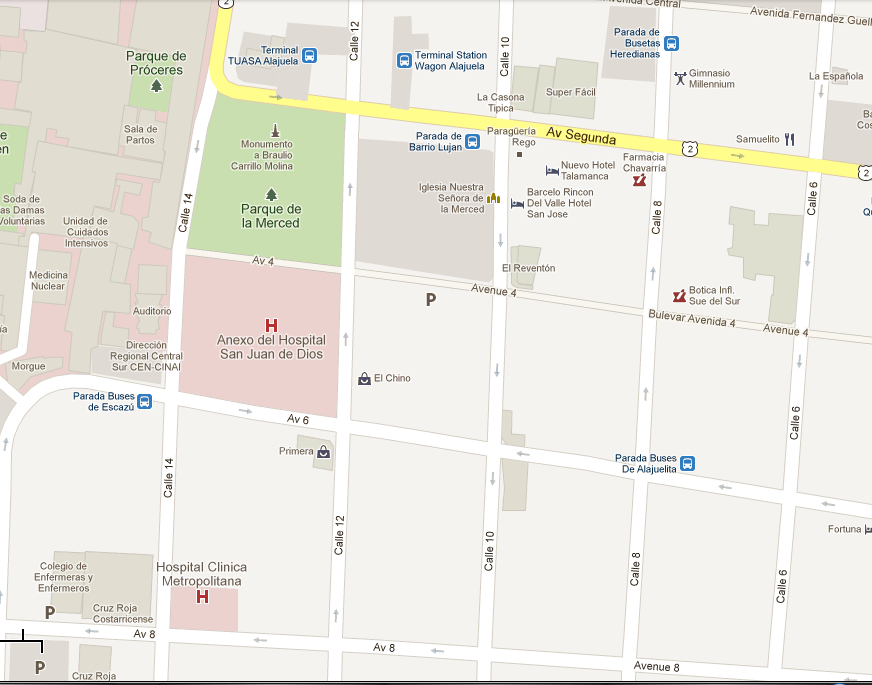
\includegraphics[totalheight=0.51\textheight]{images/trafico1}
			\caption{Diagrama de calles, San Jos\'{e} Costa Rica (Google Maps)}
			\label{fig:traficoSJ}
		\end{center}
	\end{figure}
		
		

		Basado en dicha imagen, se plantea el problema de cambio de las luces de los
	sem\'{a}foros tomando como referencia la \textbf{avenida:} 2, 4 y 8,  y las
	\textbf{calles:}
	12, 10, 8 y 6. Para este caso la avenida segunda se ve afectada fuertemente por los veh\'{i}culos automotores que quedan en medio de las intersecciones, si bien este es un problema m\'{a}s cultural, se ver\'{i}a mitigado al contar con una red de sem\'{a}foros inteligentes que tomen decisiones basados en su entorno.
	
		As\'{i} por ejemplo, al presentarse una disminuci\'{o}n del flujo de veh\'{i}culos
	automotores desde la intersecci\'{o}n de la avenida 6 y calle 10 hasta la avenida
	segunda, debido a que los sem\'{a}foros de estas est\'{a}n pasando a la luz roja,
	posiblemente se generar\'{a} una obstrucci\'{o}n en los carros que circulan a  trav\'{e}s
	de la avenida segunda. Al presentarse este escenario, muchos de los veh\'{i}culos no podr\'{a}n pasar aun cuando tengan la luz verde permiti\'{e}ndoselos.
	
		Dependiendo de las condiciones en ese momento, ya sea un alto n\'{u}mero de
	veh\'{i}culos automotores en la cercan\'{i}a o la presencia de una fuerte lluvia que
	dificulte la conducci\'{o}n, es probable que se genere un efecto en cadena el cual
	culminar\'{a} afectando, con igual o mayor rapidez, otras \'{a}reas.
	
		Otro posible escenario, es la ausencia de un n\'{u}mero significante de veh\'{i}culos
	que est\'{a}n pasando por alguna de las calles de la intersecci\'{o}n, mientras que la
	avenida se encuentra llena o a punto de saturarse por la imposibilidad de poder
	pasar debido a la luz roja, porque otro de los sem\'{a}foros est\'{a} permitiendo paso
	a  unos cuantos veh\'{i}culos que vienen por la calle. En este caso el causar que se detengan muchos automotores por permitir pasar a unos cuantos generar\'{a} un aumento en el consumo de combustible porque estos deben arrancar o pasar a bajas velocidades.
	
		En ambos casos, es notable como una mala coordinaci\'{o}n entre los sem\'{a}foros de
	una red terminan causando estragos en las calles del pa\'{i}s. Aun contando con
	sistemas de control centralizados para el manejo de estos, no se puede
	garantizar una mejora notable en el rendimiento ya que los c\'{a}lculos son
	realizados por personas y el tiempo o consideraciones que tomen estos, pueden no ser suficientes para tomar la mejor decisi\'{o}n.
	
	

	\section{Justificaci\'{o}n}

		
		Siempre ha existido el inter\'{e}s por lograr una mejora en el tr\'{a}nsito vehicular
	y se puede notar como la incorporaci\'{o}n de inteligencia artificial dentro de esta
	\'{a}rea  se ha ido incrementando con el paso de los a�os. Costa Rica, al igual que muchos pa\'{i}ses a nivel mundial, ha dado los primeros pasos para poder lograr la transici\'{o}n a estas mejoras, si bien en algunos se han logrado implementar mejores opciones, esto no siempre ha conseguido satisfacer en forma constante las necesidades de los usuarios. Muchas quejas han sido presentadas por los conductores [17] y diferentes factores inciden dentro de este tipo de problemas, desde una simple lluvia hasta desviaciones por construcciones o arreglos que se realicen aumentando las concentraciones de veh\'{i}culos en ciertos puntos.
	
		El incorporar las redes neuronales a una red de sem\'{a}foros resulta un reto,
	pero a la vez con su implementaci\'{o}n exitosa se lograr\'{a}n grandes mejoras al sistema
	de tr\'{a}nsito vehicular de los pa\'{i}ses que opten por realizar dicho proyecto.
	
		En el modelo que se posee actualmente en Costa Rica, no se dispone de alguna
	forma en que estos sem\'{a}foros funcionen de forma aut\'{o}noma mientras que al hacer
	uso de redes neuronales se dar\'{a} un gran avance en la administraci\'{o}n de estos ya
	que, como se dijo anteriormente, la red neuronal le permitir\'{a} a los sem\'{a}foros aprender y con el tiempo poder hacer predicciones del flujo de autom\'{o}viles tal y como se plantea en [3].
	
		Actualmente un sem\'{a}foro perteneciente a un sistema inteligente b\'{a}sico puede
	decidir qu\'{e} hacer, pero esta decisi\'{o}n corresponde \'{u}nicamente a lo que este
	puede observar por medio de los sensores con los que cuente, por otro lado al
	encontrarse varios sem\'{a}foros interconectados y tomando decisiones seg\'{u}n los datos que uno le indique al otro, todos podr\'{a}n contar con un panorama m\'{a}s claro y amplio de lo que realmente est\'{a} sucediendo en un nivel global.
	
		En el \'{a}rea de las redes neuronales existen una gran cantidad de modelos
	utilizados para poder implementarlas, algunos de los cuales han sido objeto de
	estudio para formar parte de alguna propuesta de sistema para el control de
	tr\'{a}fico. La tesis busca definir y  proponer una alternativa a dichos modelos, el cual permita establecer un sistema de simulaci\'{o}n para la predicci\'{o}n que administre de forma id\'{o}nea el tiempo de esperas de los autom\'{o}viles en los sem\'{a}foros mientras circulan por las calles, tomando como forma de aprendizaje la propagaci\'{o}n hacia atr\'{a}s con entrenamiento de tipo supervisado mediante la cual se obtendr\'{a} una modificaci\'{o}n que se adapte lo mejor posible al problema en cuesti\'{o}n.
	
		Cabe destacar que al realizarse la simulaci\'{o}n, se estar\'{a}n probando todos los
	aspectos sobre el modelo de red neuronal a desarrollar por lo que los
	resultados, y efectos (positivos o negativos) generados se lograr\'{a}n visualizar
	de esta forma. Por esta raz\'{o}n el esfuerzo se ver\'{a} enfocado en llegar a obtener un modelo que logre hacer bien su cometido, pero su implementaci\'{o}n en un ambiente real no forma parte de esta tesis, si no que se deja abierto para una futura realizaci\'{o}n, la cual se ver\'{a} favorecida gracias al an\'{a}lisis estad\'{i}stico de los factores que realizar\'{a} como una forma de confirmar el funcionamiento adecuado de la red con respecto al sistema actual.
	
	\subsection{Beneficios}
	
	
		El principal aporte de este trabajo consiste en brindar una alternativa a los
	modelos actuales de sistemas de sem\'{a}foros inteligentes basados en redes
	neuronales con el que se pueda contrastar las ventajas y desventajas que
	proporcionan los actuales con respecto al modelo que se proponga en la tesis.
	
		Dicho modelo al ser una alternativa, ayudar\'{a} con ideas de modificaciones que
	son posibles realizar a los modelos actuales, en los que pueden no haberse
	considerado ciertos tipos de variables debido al hecho de no estar pensados espec\'{i}ficamente para este tipo de problemas. Con esto se podr\'{a}n abrir puertas a futuras mejoras del mismo o a posibles agregados que  no fueron considerados, por alg\'{u}n motivo, como parte de esta investigaci\'{o}n.
	
		De igual forma, esta tesis ayudar\'{a} a poner en claro las mejoras que se dan en
	caso de lograr la implementaci\'{o}n de este modelo en las calles de San Jos\'{e}. Lo
	anterior se debe a la necesidad de realizar una serie de an\'{a}lisis estad\'{i}sticos
	para evaluar diferentes factores que inciden en el control del tr\'{a}fico, con la finalidad de poder saber ante qu\'{e} factores funciona bien, o no el modelo propuesto para el sistema, pero que a la vez permitir\'{a} contrastar la informaci\'{o}n estad\'{i}stica generada por el sistema actual permitiendo saber las deficiencias espec\'{i}ficas que existan del mismos.
	
		Finalmente, al contar con las comparaciones mencionadas anteriormente, el
	Centro de control de tr\'{a}nsito del MOPT podr\'{a} hacer uso de esta
	retroalimentaci\'{o}n para llevar a cabo cualquier �ajuste� que sea necesario de
	forma que se busquen mejorar las disminuciones de tiempo y poder lograr m\'{a}s del
	30\% que se ha logrado actualmente, as\'{i} como mejorar el \'{i}ndice de ahorros en
	combustible anuales superando los \$4 millones, es decir m\'{a}s de lo indicado
	en [15] y trayendo consigo una mejor respuesta y una mayor satisfacci\'{o}n de
	los conductores.
	
	
	
	

	\section{Hip\'{o}tesis}

\textit{El uso de t\'{e}cnicas de IA posibilita la realizaci\'{o}n de un sistema
de control de tr\'{a}nsito distribuido, donde se utilicen como parte de los par\'{a}metros datos
proporcionados por los mismos sem\'{a}foros y que permita administrar los tiempos de
espera empleados por los conductores y aumentar la fluidez del tr\'{a}fico.}

\section{Objetivos}
	\subsection{Objetivo General}
	
		Desarrollar y simular un modelo que permita la implementaci\'{o}n y an\'{a}lisis de un
	sistema distribuido de sem\'{a}foros inteligentes basado en redes neuronales
	artificiales, para lograr un mejor control del tr\'{a}fico que fluye
	por las zonas m\'{a}s congestionadas de San Jos\'{e}, en el que se consideren
	factores que obstruyen o alteran su flujo continuo.
	
	\subsection{Objetivos Espec\'{i}ficos}
	\begin{enumerate}
	  \item Establecer puntos de referencia sobre el funcionamiento y rendimientos,
	  que ayuden en la especificaci\'{o}n del modelo a desarrollar por medio del
	  an\'{a}lisis de los modelos actuales para la implementaci\'{o}n de sistemas
	  de sem\'{a}foros basados en redes neuronales, as\'{i} como el sistema empleado en Costa Rica.
	  
	  \item Dise\~{n}ar e implementar un modelo de red neuronal empleando
	  propagaci\'{o}n hacia atr\'{a}s (backpropagation), para el entrenamiento de
	  la red siendo uno de los modelos propuestos actualmente para la implementaci\'{o}n de un sistema de sem\'{a}foros inteligentes basado en redes neuronales.
	  \item Evaluar el desempe\~{n}o de la red neuronal en diferentes escenarios
	  basados en informaci\'{o}n estad\'{i}stica real  en
	  los que se consideren factores con diferentes niveles de incidencia que
	  influyen en el flujo normal del tr\'{a}fico veh�cular dentro del rango avenida: 2, 4 y 8,  y las calles: 12, 10, 8 y 6 de San Jos\'{e}.
	  %\item Simular escenarios cambiantes en los que se incluyan factores en sus
	  %diferentes niveles que afecten el tr\'{a}fico, donde se consideren eventos
	  % t\'{i}picos (alto n\'{u}mero de veh\'{i}culos), as\'{i} como los poco frecuentes (colisiones, carros varados, presencia de lluvia, reparaciones de v\'{i}as) dentro del rango avenida: 2, 4 y 8,  y las calles: 12, 10, 8 y 6 de San Jos\'{e}.
	  \item Contrastar los ambientes vividos y factores que se presentan en las
	  principales zonas de San Jos\'{e}, por medio de an\'{a}lisis estad\'{i}stico para poder contrastar los resultados obtenidos por el uso de la red neuronal contra los datos reales que ha generado actualmente el sistema de control de tr\'{a}fico.
	  \item Entrenar la red neuronal artificial hasta obtener mejoras en el
	  desempe\~{n}o por medio de un proceso iterativo de simulaciones el
	  cual permita mejorar los c\'{a}lculos realizados por redes neuronales aplicado a los diferentes factores del experimento, tomando como base de comparaci\'{o}n los datos actuales generados por el sistema de control de tr\'{a}fico para lograr diferencias notables en la administraci\'{o}n de tiempos en los sem\'{a}foros.
	  
	\end{enumerate}

	\section{Alcance y Limitaciones}
		
		
		Esta tesis se enfocar\'{a} a las situaciones ocurridas \'{u}nicamente en San Jos\'{e}
	dentro de las zonas en las que opera actualmente el sistema de control de
	tr\'{a}fico, primero en la ciudad de San Jos\'{e} en las \textbf{avenida:} 2, 4
	y 8,  y las \textbf{calles:} 12, 10, 8 y 6; que ser\'{a} tomada como base inicial para el
	desarrollo y entrenamiento de la red neuronal.
	
		Adicionalmente, se elaborar\'{a} una red neuronal que funcione en un m\'{i}nimo de
	seis sem\'{a}foros ubicados en diferentes intersecciones de la zona delimitada
	anteriormente. Estos tomar\'{a}n las decisiones en conjunto para administrar y
	coordinar los tiempos que deben permanecer en luz verde o cuando es necesario
	que uno o varios de estos cambien a luz roja. Se realizar\'{a} varias
	simulaciones ya que se busca determinar bajo qu\'{e} factores funciona mejor el
	sistema mencionado, para esto, los datos que se obtengan como resultado del
	funcionamiento de la red ser\'{a}n valorados con respecto a las bit\'{a}coras
	que sean proporcionadas por el \textit{Centro de Control de Tr\'{a}fico del
	MOPT}.
	Cabe destacar que s\'{o}lo se proceder\'{a} a hacer pruebas en otras regiones de San Jos\'{e} hasta obtener resultados confiables de las pruebas realizadas en las zonas descritas.
	
		Como parte de las labores requeridas, se crear\'{a} un programa para simular los
	escenarios planteados para entrenamiento y prueba de la red neuronal. No se
	tomar\'{a}n como par\'{a}metro de entrada el consumo de combustible de los autom\'{o}viles,
	ni los gastos relacionados con estos. De igual forma, no se validar\'{a}n las
	entradas que reciba la red, es decir, todos los datos presentados a la red ser\'{a}n correctos sin consideraciones de alg\'{u}n tipo que afecte a las entradas de la red. Tampoco se contempla la implementaci\'{o}n y pruebas correspondientes en un ambiente real, esto debido a que el centro de control de tr\'{a}fico no dispone de recursos para intervenir en la realizaci\'{o}n de esto. No obstante, la funcionalidad y resultados podr\'{a}n ser apreciados por medio del programa de simulaci\'{o}n mencionado, por lo que el esfuerzo se centra m\'{a}s en definir, desarrollar y probar el modelo de red neuronal que logre hacer su cometido de la mejor forma posible.
	
		El no contar con los sensores necesarios para la detecci\'{o}n de veh\'{i}culos
	automotores  as\'{i} como el presupuesto para adquirirlo, se convierte en una de
	las principales limitantes por las cuales el modelo no ser\'{a} implementado en un
	ambiente real. De igual forma, no se cuenta con el personal y tiempo necesarios para llevar a cabo esta labor, ya que el tiempo establecido para la realizaci\'{o}n de este trabajo podr\'{i}a no ser suficiente para llevar a cabo ambas labores, es decir, tanto el desarrollo del modelo como la implementaci\'{o}n en un ambiente real del mismo.
		
		La implementaci\'{o}n del modelo resultado de esta tesis se deja como tema para su
	posterior realizaci\'{o}n en otro trabajo, motivando a otras personas a retomar la
	soluci\'{o}n y brindar sus propios aportes y mejoras al mismo.\\

\section{Lista de Entregables}

Como parte de realizaci\'{o}n de la tesis se realizar\'{a} un modelo alternativo
que utilice el algoritmo de propagaci\'{o}n hacia atr\'{a}s para su
entrenamiento y la documentaci\'{o}n correspondiente. Lo cual se divide en los
siguientes entregables:

\begin{itemize}
  \item Algoritmo para la programaci\'{o}n de la red: En el lenguaje y
  plataformas especificados previamente. \'{E}ste consistir\'{a} de la
  l\'{o}gica de su implementaci\'{o}n, y los archivos en el lenguaje de
  programaci\'{o}n seleccionados.
  \item Programa de simulaci\'{o}n de escenarios para la red  neuronal: este
  programa ser\'{a} empleado para poder realizar pruebas a la red, de forma que
  se puedan realizar los ajustes necesarios para que esta cometa la menor
  cantidad de errores posibles. Para este se tomar\'{a}n en cuenta los factores
  que afectan el desempe\~{n}o de la red.
  \item Documentaci\'{o}n del an\'{a}lisis estad\'{i}stico de los resultados obtenidos al
  entrenar la red neuronal, de forma que se pueda determinar bajo cu\'{a}les
  condiciones esta funciona mejor. De igual forma se contempla una
  comparaci\'{o}n con respecto a los tiempos de cambios de luces obtenidos del
  sistema actualmente utilizado por el Centro de Control de Tr\'{a}fico del
  MOPT.
  \item Datos obtenidos de las pruebas realizadas a la red neuronal: estos datos
  corresponden a los resultados finales sobre los ajustes que fueron hechos
  sobre la red, los errores que se corrigieron y su evaluaci\'{o}n con respecto
  al criterio de validez para determinar los valores reales esperados.
\end{itemize}

\section{Beneficios Esperados}
	
			Esta tesis ayudar\'{a} a poner en claro las mejoras que se dan en
	caso de lograr la implementaci\'{o}n de este modelo en las calles de San Jos\'{e}. Lo
	anterior se debe a la necesidad de realizar una serie de an\'{a}lisis estad\'{i}sticos
	para evaluar diferentes factores que inciden en el control del tr\'{a}fico, con
	la finalidad de poder saber ante qu\'{e} factores funciona bien, o no el modelo
	propuesto para el sistema, pero que a la vez permitir\'{a} contrastar la
	informaci\'{o}n estad\'{i}stica obtenida del sistema actual permitiendo
	saber las deficiencias espec\'{i}ficas que existan del mismos.
	
		Por otro lado, al contar con las comparaciones mencionadas anteriormente, el
	Centro de control de tr\'{a}nsito del MOPT podr\'{a} hacer uso de esta
	retroalimentaci\'{o}n para llevar a cabo cualquier �ajuste� que sea necesario de
	forma que se busquen mejorar las disminuciones de tiempo y poder lograr m\'{a}s del
	30\% que se ha logrado actualmente, as\'{i} como mejorar el \'{i}ndice de ahorros en
	combustible anuales superando los \$4 millones, es decir m\'{a}s de lo indicado
	en [15] y trayendo consigo una mejor respuesta y una mayor satisfacci\'{o}n de
	los conductores.
	
		Para el caso del investigador, se espera obtener conocimientos m\'{a}s amplios
	sobre las redes neuronales, buenas pr\'{a}cticas involucradas dentro de la
	realizaci\'{o}n de sistemas de control de tr\'{a}nsito en general y
	especialmente los que se basen o hagan uso de redes neuronales. Con esto se
	pretende llegar a obtener conocimientos mayores a los que haya dejado la
	carrera de Ingenier\'{i}a en Sistemas de Informaci\'{o}n y poder abarcar temas
	que exigan un aprendizaje, y no s\'{o}lo la puesta en pr\'{a}ctica de
	de temas vistos durante la carrera.

		Por \'{u}ltimo, para la Universidad Nacional se busca incentivar la
	realizaci\'{o}n de tesis o proyectos que se inclinen m\'{a}s por la
	investigaci\'{o}n donde se involucren temas que no se basen en asuntos,
	soluciones comunes o se limiten a la realizaci\'{o}n de otro sistema. Se
	espera lograr que la misma universidad sea la encargada de motivar a los
	aspirantes a indigar sobre temas nuevos que resulten retadores por el grado de
	complejidad que implican, pero que al final dejen un gran aporte en diferentes
	\'{a}reas y que ayuden a obtener investigaciones de gran calidad.
	

	

\chapter{Marco Te\'{o}rico}
	\label{chap:theory}
	
	\section{Redes neuronales y la toma de decisiones}
\subsection{El Modelo Biol\'{o}gico}
 
 		El sistema de procesamiento de informaci\'{o}n completo est\'{a} formado en parte el
 	sistema nervioso central cuyo elemento principal es el cerebro. \'{e}ste a su vez
 	se encuentra compuesto por una unidad fundamental llamada \textit{neurona}.
 	\cite{Kriesel2005} La figura \ref{fig:neuronaBio} muestra las partes de la
 	neurona. En esta se puede observar la estructura t\'{i}pica de una neurona biol\'{o}gica, la
 	cual se encuentra formada por un cuerpo celular con su n\'{u}cleo o
 	\textit{soma}, del cual se desprende, en la parte superior, una serie de
 	ramificaciones denominadas \textit{dendritas}, mientras que en la parte
 	inferior se puede observar el \textit{ax\'{o}n}, \'{e}ste es una extensi\'{o}n del soma de forma tubular y
 	tiende a ramificarse en uno de sus extremos.
 	
 	\begin{figure}[htp]
 		\centering
 		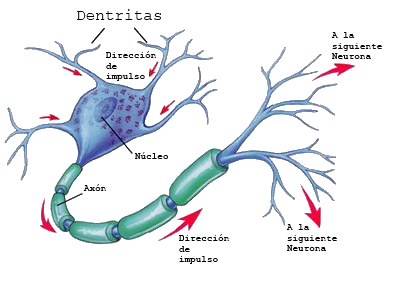
\includegraphics[width=0.5\textwidth]{images/TesisYGR-neuron.png}
 		\caption{Neurona Biol\'{o}gica}
 		\label{fig:neuronaBio}
 	\end{figure}
 	
 	 		Las neuronas son como cualquier otro tipo de c\'{e}lula, con la diferencia que
 	\'{e}stas pueden comunicarse entre s\'{i} \cite{Longo2011}. Por lo anterior, las dendritas
 	funcionan como una canal de entrada para recibir las se\~{n}ales que provienen del
 	exterior. Estas se\~{n}ales se transfieren a una neurona por medio de una conexi\'{o}n o contacto denominado sinapsis, mientras que el ax\'{o}n transfiere los pulsos hacia otras neuronas.

		Las se\~{n}ales entre las neuronas pueden ser de tipo el\'{e}ctrica o sinapsis
	el\'{e}ctrica que se da cuando la sinapsis recibe una se\~{n}al el\'{e}ctrica proveniente
	de una neurona transmisora o neurona pre sin\'{a}ptica y este es transmitido al
	n\'{u}cleo de la neurona receptora o pos sin\'{a}ptica. Por otro lado la sinapsis qu\'{i}mica se distingue por no presentarse un contacto el\'{e}ctrico entre ambas partes ya que este se interrumpe por causa de un abismo o grita sin\'{a}ptico que separa un lado del otro. No obstante la informaci\'{o}n siempre fluye debido a que la se\~{n}al el\'{e}ctrica en el lado pre sin\'{a}ptico de la grita se convierte en una se\~{n}al qu\'{i}mica que atraviesa la grieta y luego se vuelve a convertir en el la receptor \cite{Kriesel2005}.
 	
 		Una caracter\'{i}stica adicional de la sinapsis es la intensidad con la que se
 	transmiten las se\~{n}ales ya que estas tienden a variar, siendo unas transferidas
 	con fuerte estimulaci\'{o}n mientras que otras de forma d\'{e}bil. Este ajuste varia
 	permitiendo que la estructura del cerebro no se mantenga fija formando conexiones m\'{a}s fuertes o d\'{e}biles seg\'{u}n se requieran ajustes.

 		Usando un punto de vista funcional, una neurona de forma aislada, se
 	constituye en un procesador b\'{a}sico de informaci\'{o}n que cuenta con secci\'{o}n para
 	entradas (dendritas), un \'{a}rea de procesamiento (n\'{u}cleo o soma) y secci\'{o}n de
 	salida. Con forme se aumenta el panorama se y se incluyen m\'{a}s neuronas y las interconexiones entre estas, se obtiene una red de neuronas que usan la sinapsis para poder transmitir se\~{n}ales unas a otras.
 		
 		

	\section{Redes neuronales artificiales}
		
		
		El cerebro humano es tan sorprendente que se ha tratado de imitar a trav\'{e}s de
	la tecnolog\'{i}a. Las redes neuronales artificiales representan una forma
	funcional y estructural de esta b\'{u}squeda por imitar el cerebro humano. Tal como
	su nombre lo indica, estas redes son una emulaci\'{o}n del comportamiento de una red neuronal biol\'{o}gica, pero diversos autores las definen de cierta forma particular por lo que a continuaci\'{o}n se mencionan algunas de ellas.
	
	\begin{itemize}
	  \item Un modelo que surgi\'{o} para emular el proceso de aprendizaje es la red
	  neuronal artificial. Las redes neuronales son modelos que intentan reproducir
	  el comportamiento del cerebro humano. \cite{Hilera1995}
	  \item Las redes neuronales artificiales son, lo que su nombre indica,
	  redes computacionales que intentan simular, las redes de c\'{e}lulas nerviosas o
	  neuronas del sistema nervioso central del ser humano. \cite{Graupe2007}
	\end{itemize}
	
		Como se puede observar, las redes neuronales han obtenido buenos resultados en
	los procesos de aprendizaje y formando parte de procesos de an\'{a}lisis. De
	acuerdo con Kumar \cite{Kumar2007}, estas redes poseen la capacidad de
	generalizar y por lo tanto pueden predecir nuevos resultados a partir de resultados previos, y de igual forma pueden procesar informaci\'{o}n en paralelo a altas velocidades y de forma distribuida.
	
		Por las razones anteriores, se plantea la tesis entorno al uso de una red
	neuronal para lograr una toma de decisiones en una red formada por sem\'{a}foros.
	
		En este caso como se tiene un objetivo muy claro, por lo que resulta posible
	utilizar un modelo de propagaci\'{o}n hacia atr\'{a}s (backpropagation), este es uno
	de los m\'{a}s empleados para la implementaci\'{o}n de las redes neuronales, por lo
	que ser\'{a} tomado como base para el entrenamiento de la red a implementar con
	el modelo propuesto para esta tesis. De igual forma se ver\'{a} el contraste
	que se pueda obtener con respecto al modelo de Hopfield mencionado por Gilmore
	y Elibiary \cite{Gilmore1993}, como una de las opciones m\'{a}s viables para la
	realizaci\'{o}n de este tipo de sistemas.

% 	\subsection{Componentes de una red neuronal}
% 	
% 		Al tratar de imitar a sus contrapartes biol\'{o}gicas, las redes neuronales
% 	artificiales llevan consigo una serie de componentes los cuales resultan
% 	importantes destacar para su posterior implementaci\'{o}n.
% 	
% 	\begin{itemize}
% 	  \item \textbf{Vector de entrada:} corresponde a las entradas provenientes de
% 	  cada neurona conectada.
% 	  \item \textbf{Escalar de salida:} la salida de la red resulta un \'{u}nico valor
% 	  escalar, debido a que durante el procesos las entradas son acumuladas.
% 	  \item \textbf{Cambio de entradas en la sinapsis:} las entradas son procesadas
% 	  por medio de la multiplicaci\'{o}n del peso asociado a la conexi\'{o}n.
% 	  \item \textbf{Acumulaci\'{o}n de entradas:} tanto las redes biol\'{o}gicas
% 	  como las artificiales suman las entradas permitiendo as\'{i} obtener un resultado para la neurona.
% 	  \item \textbf{Pesos ajustables:} Los pesos que cambian el valor de las
% 	  entradas a una neurona son ajustables, agregando de esta forma dinamismo a la red debido a que gran parte del conocimiento de una red se encuentra almacenada en sus pesos.
% 
% 	\end{itemize}
% 
% 		A pesar de las definiciones dadas sobre redes neuronales, no se ha dado una
% 	que refleje la verdadera forma conceptual de la misma, por eso de  acuerdo con
% 	\cite{Kriesel2005}:
% 	
% 		\textit{Una red neuronal es una tripleta ordenada $(N,V,w)$ con dos conjuntos
% 		N, V y una funci\'{o}n w.}
% 	
% 	Donde:
% 	\textbf{N} es el conjunto de neuronas
% 	\textbf{V} es un conjunto $\lbrace(i,j) | i, j 2 \in N\rbrace$  cuyos elementos
% 	son llamados conexiones entre las neuronas, i y j 
% 	\textbf{W} es una funci\'{o}n $w: V\to\mathbb{R}$ que define los
% 	pesos, los valores indefinidos o 0 se dejan para las conexiones que no existen dentro de la red.
% 	
% 	
% 		Adicionalmente cada neurona cuenta con una serie de funciones para el manejo
% 	de las entradas, procesamiento de las mismas y la generaci\'{o}n de su salida. Estas
% 	corresponde a:
% 
% 	\begin{itemize}
% 	  \item \textbf{Funci\'{o}n de propagaci\'{o}n:} como ya sabe cada neurona se
% 	  encuentra conectada otras neuronas, por esta raz\'{o}n para la neurona $j$ se
% 	  van a recibir n entradas, eso se recibe en forma de un vector de entrada con
% 	  la informaci\'{o}n proveniente de cada una de estas. M\'{a}s detalladamente,
% 	  esta se encarga de recibir las entradas $O_{i_1},\ldots, O_{i_n}$
% 	  provenientes de las neuronas $i_1,\ldots,i_n$ las cuales forman el conjunto
% 	  $I = \lbrace i_1,\ldots,i_n\rbrace $, y que se encuentran conectadas a la
% 	  neurona $j$, luego de esto, la funci\'{o}n de propagaci\'{o}n convierte ese vector de entrada en un \'{u}nico escalar conocido como entrada de la red o
% 	  $net_j$. 
% 	  
% 	  \begin{equation}
% 	  	net_j = f_{prop}(o_{i_1},\ldots,o_{i_n} , w_{i_1,j},\ldots,w_{i_n,j})
% 	  \end{equation}
% 	  
% 	  Por lo general se emplea una sumatoria de las entradas por los pesos
% 	  de las conexiones obteniendo como resultado el escalar mencionado.
% 	  
% 	  \begin{equation}
% 	  	net_j = \sum_{i \in I} (o_i \cdot w_{i,j})
% 	  \end{equation}
% 	 
% 	  \item \textbf{Funci\'{o}n de activaci\'{o}n:} esta funci\'{o}n se encarga de
% 	  cambiar el estado de activaci\'{o}n de la neurona. En otras palabras, para
% 	  una neurona $j$,  el estado de activaci\'{o}n $a_j$ se asigna a la neurona
% 	  como resultado de la funci\'{o}n indicando de esta forma el grado de actividad de la misma.
% 	  
% 	  Cabe destacar que las neuronas se ven activadas si la entrada de la red
% 	  excede el umbral establecido. En este caso una neurona $j$, el valor del
% 	  umbral $\Theta_j$ se asigna de forma \'{u}nica a $j$,  marcando de esta forma el
% 	  gradiente de valor m\'{a}ximo de la funci\'{o}n de activaci\'{o}n.
% 	  
% 	  		\begin{equation}
% 	  			a_j(t) = f_{act}(net_j(t)),a_j(t-1),\Theta_j)
% 	  		\end{equation}
% 	  
% 	  Esto transforma la entrada de la red $net_j$ y el estado de activaci\'{o}n
% 	  anterior $a_j(t - 1)$ en el nuevo estado de activaci\'{o}n $a_j(t)$
% 	  
% 	  
% 	  \item Funci\'{o}n de salida: se encarga de calcular el valor que ser\'{a}
% 	  transmitido a las otras neuronas conectadas a $j$. Por lo general se hace uso
% 	  de la funci\'{o}n identidad en otras palabras, el valor $a_j$ para la
% 	  activaci\'{o}n se coloca directamente como la salida.
% 	\end{itemize}
% 	
% 	
% 	\subsection{Topolog\'{i}as}
% 	
% 		La topolog\'{i}a de las redes neuronales consiste en la arquitectura o forma en la
% 	que se organizar\'{a}n las neuronas dentro de la red, forman de esta forma una
% 	serie de capas o agrupaciones que sin importar los par\'{a}metros con los que se
% 	defina esta, podr\'{a} contar con tres tipos de neuronas artificiales:
% 	
% 	\begin{itemize}
% 	  \item \textbf{Neuronas de entrada:} encargadas de recibir la informaci\'{o}n
% 	  directamente desde el exterior.
% 	  \item	\textbf{Neuronas ocultas:} reciben informaci\'{o}n desde otras
% 	  neuronas.
% 	  En estas neuronas es donde se realiza la representaci\'{o}n de la informaci\'{o}n almacenada.
% 	  \item \textbf{Neuronas de salida:} toman la informaci\'{o}n procesada
% 	  devolvi\'{e}ndola al exterior.
% 	\end{itemize}
% 	
% 		Dependiendo de como se agrupen las neuronas a sea por capas o que se
% 	encuentren m\'{a}s o menos cercas de la entrada y salida de la red, se cuenta par\'{a}metros
% 	fundamentales para estas dentro de los cuales se mencionan
% 
% 	\begin{itemize}
% 	  \item El grado de conectividad
% 	  \item El tipo de conexiones existentes entre las neuronas.
% 	\end{itemize}
% 	
% 		Como punto de partida se cuenta con la redes de \textit{conexiones hacia
% 		adelante} o \textit{Feedforward}, en esta las redes se ven agrupadas en tres
% 		capas principales: una capa de entrada, $n$ capas de procesamiento escondidas
% 		y una capa de salida. Tal y como su nombre lo indica, las neuronas en tipo de red s\'{o}lo cuentan con
% 	conexiones directas con las neuronas de la siguiente capa (hacia la capa de
% 	salida). Es importante mencionar que una variante de este puede contar con conexiones de atajo o \textit{shortcuts}  para saltar una o m\'{a}s capas pero que de igual forma deben de seguir hacia adelante.
% 	
% 		Extendiendo la funcionalidad mencionada en la descripci\'{o}n anterior, se cuenta
% 	con las redes recurrentes estas permiten realizar conexiones ya sea a s\'{i} mismas
% 	conocido como \textit{recurrencia directa} o que se permitan conexiones
% 	dentro de la misma capa para una red de una o varias capas, en la denominada
% 	\textit{recurrencia lateral}. Este tipo de conexiones resultan muy \'{u}tiles
% 	en casos en los que se cuenta con una \'{u}nica capa, pero de igual forma es aplicable en el caso de m\'{u}ltiples capas.
% 	
% 		Finalmente, est\'{a}n las redes completamente conectadas las cuales permiten
% 	conexiones entre todas las neuronas con excepci\'{o}n de recurrencias directas,
% 	como resultado de este tipo e conexiones cada neurona puede convertirse en una
% 	neurona de entrada.
% 	
% 	\subsection{Activaci\'{o}n de Neuronas}
% 		De acuerdo con Kriesel \cite{Kriesel2005}, resulta muy importante el orden en el que cada
% 	neurona de forma individual recibe y procesa las entradas y genera las salidas
% 	en este se distinguen dos modelos la forma s\'{i}ncrona y la as\'{i}ncronas. Para el
% 	caso del primero, todas las neuronas cambian sus valores de forma simult\'{a}nea calculando las entradas de la red, la activaci\'{o}n de las mismas y la salida generada adem\'{a}s de ir pasando estos resultados. Este modelo es el que m\'{a}s se asemeja a la contraparte biol\'{o}gica y es el m\'{a}s gen\'{e}rico.
% 	
% 			Con respecto al modelo as\'{i}ncrono, las neuronas cambian sus valores en
% 	diferentes puntos del tiempo, por lo que existen \'{o}rdenes diferentes en las que
% 	esto puede ocurrir. Dentro de estos destacan:
% 	
% 	\begin{itemize}
% 	  \item \textbf{Orden aleatorio:} se escoge al azar una neurona $i$ para que se
% 	  actualicen sus valores $net_i, a_i y o_i$. Como es de esperarse, al no tener
% 	  un orden establecido, puede ocurrir casos en los que una neurona se escoja repetidamente durante un ciclo y otras que del todo no sean elegidas.
% 	  \item \textbf{Permutaci\'{o}n aleatoria:} se garantiza que cada neurona sea
% 	  escogida una \'{u}nica vez por cada ciclo, pero sin un orden definido. Este orden de activaci\'{o}n no es muy usado por el hecho de tener que invertir tiempo calculando una nueva permutaci\'{o}n por cada ciclo.
% 	  \item \textbf{Orden topol\'{o}gico:} las neuronas se activan de acuerdo con
% 	  un orden definido por la topolog\'{i}a. Tomando como ejemplo una red
% 	  \textit{feedforward}, las neuronas de entrada se activar\'{i}an primero,
% 	  seguidas por las neuronas ocultas y finalmente las neuronas de salida
% 	  
% 	\end{itemize}
% 	
% 	
% 	
% 	\subsection{Aprendizaje y entrenamiento}
% 	
% 	
% 		Definidos los puntos anteriores, y una vez seleccionada la topolog\'{i}a, la
% 	activaci\'{o}n de las neuronas y el tipo de neurona a utilizar, es necesario
% 	determinar la forma de entrenamiento. Como requisito para poder utilizar una red neuronal artificial, es necesario entrenarla y para realizar esto, se toma como punto de partida un conjunto de pesos aleatorios haciendo que el proceso de aprendizaje busque los pesos que permitan desarrollar de forma adecuada la tarea encomendada a la red. Este proceso esta conformado por una serie de pruebas iterativas mediante las cuales se van ajustando los componentes seg\'{u}n el desempe\~{n}o obtenido hasta lograr un nivel de resultados aceptable.
% 	
% 		Considerando lo anterior, una red neuronal puede aprender debido a alguna de
% 	las siguientes razones:
% 	
% 	\begin{itemize}
% 	  \item Desarrollo de una nueva conexi\'{o}n
% 	  \item Eliminar conexiones existentes
% 	  \item Cambio de los peso de conexiones
% 	  \item Cambio de los valores de umbral en las neuronas
% 	  \item Variaci\'{o}n de alguna de las tres funciones de la neurona (activaci\'{o}n,
% 	  propagaci\'{o}n y salida)
% 	\end{itemize}
% 	
% 	
% 	Existen varios tipos de aprendizajes de los cuales resulta importante mencionar
% 	dos:
% 	
% 	\begin{itemize}
% 	  \item \textbf{Aprendizaje supervisado:} requieren que se les brinden una
% 	  serie de datos clasificados, es decir, cada patr\'{o}n de entrada empleado para su
% 	  entrenamiento se encuentra asociado con un patr\'{o}n de salida esperado [11].
% 	  Este tipo de tipo de aprendizaje presenta la ventaja de poder optimizar los par\'{a}metros para que la red cometa la menor cantidad de errores posibles, adem\'{a}s de que al conocer las entradas y sus salidas, es posible determinar con precisi\'{o}n la cantidad de errores que se est\'{a}n cometiendo.
% 	  
% 	  Por otro lado se presenta la desventaja de tener que con una base de datos
% 	  para que el aprendizaje pueda funcionar de forma correcta, con el problema de poseer una escalabilidad limitada, es decir, se vuelven m\'{a}s lentas conforme aumenta la red.
% 	  
% 	  \item  \textbf{Aprendizaje no supervisado o auto organizado:} estas no usa un
% 	  ''maestro'' el cual les indique una clasificaci\'{o}n correcta, por lo
% 	  tanto tampoco poseen retroalimentaci\'{o}n sobre esta [12]. Este tipo de aprendizaje se asemeja m\'{a}s al aprendizaje que emplea el cerebro, contrario al aprendizaje supervisado. Otra ventaja que este brinda es que solo requiere los patrones de entrada y no se requiere realizar la clasificaci\'{o}n de los mismos. Por otro lado al indicarse la salida correcta, la red va a seguir generando resultados pero estos pueden no resultar los correctos o m\'{a}s adecuados para el problema evaluado. [21]
% 
% 	\end{itemize}
% 	
% 	
% 	De acuerdo con Ram\'{i}rez [24], el proceso de aprendizaje permite a la red
% neuronal realizar cambios a sus pesos para poder responder a las entradas que
% se le proporcionen. Dichos cambios se traducen a destrucci\'{o}n, modificaci\'{o}n o
% creaci\'{o}n de conexiones.
% 	
% 	El mismo autor resalta que: \begin{quote}\textit{``Durante el proceso de
% 	aprendizaje, los pesos de las conexiones de la red sufren modificaciones, por tanto se puede afirmar que
% este proceso ha terminado o `ha aprendido' cuando los valores de los pesos
% permanecen estables o el margen de error es menor o igual al que se ha definido
% como aceptable.''}\end{quote}(Ram\'{i}rez, 2012)
% 	
% De acuerdo con Kriesel [\cite{Kriesel2005} El objetivo principal es cambiar los valores de
% los pesos de tal forma que la red no s\'{o}lo asocie los patrones para valores de
% entrada y salida aprendidos durante el entrenamiento, sino que tambi\'{e}n provea
% resultados a patrones desconocidos o similares, otorg\'{a}ndole as\'{i} la
% capacidad de \textit{generalizar} resultados. Es por estar raz\'{o}n que resulta
% importante conocer c\'{o}mo se modifican dichos valores, definir los criterios a emplear para cambiarlos para lograr que la red aprenda una nueva informaci\'{o}n. [24]
% 
% Dichos criterios determinan la \textit{regla de aprendizaje} para la red. En
% esta se consideran dos tipos: el aprendizaje supervisado y el aprendizaje no
% supervisado, ambos mencionados anteriormente. Junto a estos se a\~{n}ade el momento
% en el cual la red puede \textit{``aprender''} ya sea durante su funcionamiento
% (online) o fuera de este mientras se encuentra desconectada (offline).
% 
% Tanto el entrenamiento online como el offline presentan sus ventajas y
% desventajas, en el caso del aprendizaje online la red aprende de forma directa
% de los errores obtenidos de los resultados alterando los pesos de forma din\'{a}mica
% siempre y cuando se le presenten o posee informaci\'{o}n nueva para procesar, lo
% anterior causa que no se distinga entre fase de entrenamiento y de
% operaci\'{o}n. Por su lado, el aprendizaje offline, tambi\'{e}n denominado \textit{entrenamiento en lote}  posee una fase de aprendizaje o entrenamiento y una fase de operaci\'{o}n bien definidas. Contrario al entrenamiento online, los pesos permanecen fijos una vez que se haya terminado la fase de entrenamiento y no cambiar\'{a}n hasta no llevar acabo otra.
% 
% 
% \subsection{Supervisi\'{o}n de un red neuronal}
% 
% 	Mientras una red no haya terminado su entrenamiento se hace uso de una
% correcci\'{o}n de error para lograr obtener resultados adecuados. Kriesel \cite{Kriesel2005}
% brinda tres definiciones involucradas en el proceso, estas corresponden a los
% patrones de entrenamiento (training pattern), entradas de ense\~{n}anza (teaching input) y el vector de error o vector de diferencia (error vector).
% 
% 	Los \textit{patrones de entrenamiento} corresponden simplemente a un vector de
% 	entrada, del cual se conoce su respectiva salida. Por su parte, las entradas de
% ense\~{n}anza consisten de un vector de salida deseado para los patrones de
% entrenamiento proporcionados previamente. Finalmente, el vector de error es la diferencia entre el vector de salida esperado (entradas de ense\~{n}anza) y el resultado obtenido.
% 
% 	En [24] Ram\'{i}rez menciona una t\'{e}cnica para corregir el error cometido por la
% red, la cual consiste de los siguientes pasos:
% 
% \begin{enumerate}
%   \item Inicializar los pesos de la red con valores aleatorios
%   \item Presentar un patr\'{o}n de entrada y propagaci\'{o}n de los valores hasta
%   calcular la salida.
%   \item Adaptar los pesos basados en el error cometido teniendo en cuenta la
%   salida esperada. Llevando a cabo el procedimiento mientras no se obtenga un error menor o igual al error aceptado.
% \end{enumerate}	

%\subsection{Algoritmo de Backpropagation}

	El algoritmo que se mencion\'{o} anteriormente (backpropagation), corresponde a
	una de las diferentes t\'{e}cnicas de aprendizaje que se pueden utilizar en una
	red neuronal. M\'{a}s detalladamente, es un m\'{e}todo de aprendizaje
	supervisado que consta de dos fases: en la primera se aplica un patr\'{o}n de entrada el cual se propaga por toda la red a trav\'{e}s de
las distintas capas de esta generando de esta forma una salida. Una vez obtenido
el resultado, se compara contra la salida deseada y se calcula el error cometido
por cada una de las neuronas de salida. Luego se transmite el conjunto de
errores hacia atr\'{a}s en este caso tomando como punto de partida la capa de
salida hacia el resto de neuronas localizadas en las capas intermedias
\cite{Fritsch1996}. Cabe destacar que el error recibido por cada neurona es
proporcional a su contribuci\'{o}n sobre el error total causado en la red. Por lo que tom\'{a}ndose dicho error como base se realizan ajustes a los pesos de las conexiones o pesos sin\'{a}pticos de cada neurona.

\subsection{Sistemas Expertos vs Redes Neuronales}
 
 		Como alternativa para la toma de decisiones se encuentran los sistemas
 	expertos, estos se caracterizan por contar con una base de conocimiento que
 	se encuentra separada del sistema original, permitiendo agregar nuevo
 	conocimiento a este sin requerirse realizar cambios al sistema. No obstante, se necesita una persona experta en un \'{a}rea para que se puedan crear las reglas que codifiquen el conocimiento \cite{Basogain}.
 	
 		Basogain en su escrito resalta las ventajas de las redes neuronales sobre
 	estos sistemas al descatar que el desarrollo de una red neuronal no se
 	requiere programar ni el conocimiento ni las reglas para procesar ese
 	conocimiento, ya que es ella misma la que aprende las reglas mediante los ajustes que se realicen a las conexiones entre las neuronas.
 		
 		Un sistema experto hace expl\'{i}cito su conocimiento en forma de reglas pre
 	establecidas, mientras que las redes neuronales generan sus reglas
 	aprendiendo, usando como materia prima los ejemplos que le fuesen mostrados
 	durante la fase de entrenamiento de la red.
 		
 			La forma en que los sistemas expertos almacenan la informaci\'{o}n se ve opacada
 	por el modo empleado en las redes neuronales, ya que estas guardan su
 	conocimiento de forma distribuida a lo largo de la red y no en una sola base
 	centralizada. La caracter\'{i}stica anterior resulta una gran ventaja debido a que se pueden usar de forma asociativa, es decir, si s\'{o}lo reciben una entrada parcial la red determinar\'{a} la entrada m\'{a}s parecida en memoria y dar\'{a} una salida asociada con la entrada original completa, concedi\'{e}ndoles la capacidad de generalizar, mientras que un sistema experto requiere de la entrada completa para poder determinar la soluci\'{o}n de acuerdo a su base de conocimiento.

 		Finalmente, se encuentra la tolerancia a fallos, el cual se refiere al caso
 	de que si fallan partes de las neuronas simplemente se realizar\'{a}n
 	modificaciones a las conexi\'{o}n, variando \'{u}nicamente su comportamiento
 	pero el sistema en cuesti\'{o}n no deja de funcionar. Con esto queda claro que
 	las redes neuronales se desempe\~{n}an mejor, por lo cual se adec\'{u}an
 	m\'{a}s para solucionar el problema presentado en esta tesis.
 	
%  		Luego de exponer las caracter\'{i}sticas de ambos elementos, se puede observar
%  			que a pesar de existir alternativas como los sistemas expertos, las redes neuronales se desempe\~{n}an mejor en los procesos de aprendizaje, en reconocer patrones y generalizar, motivos por los cuales fueron elegidas para la soluci\'{o}n propuesta con esta tesis.


	\section{Sistemas de Transporte Inteligente}

	Ezell \cite{Ezell2010}  pone en claro el hecho de que las Tecnolog\'{i}as de la
	Informaci\'{o}n han permitido obtener avances en el control de los sistemas de transportes al
permitir que los elementos de este -�veh\'{i}culos, caminos luces de
tr\'{a}fico, se\~{n}ales de mensajes, entre otras- se vuelvan inteligentes al emplear chips
embebidos, as\'{i} como sensores que les permitan comunicares unos con otros por
medio del uso de tecnolog\'{i}as cableadas o inal\'{a}mbricas. Los sistemas de
transportes inteligentes o \textit{Intelligent Transportation Systems} (ITS) que se han implementado a nivel mundial, han tra\'{i}do consigo mejoras significativas al desempe\~{n}o del sistema de transporte, el cual abarca no s\'{o}lo reducci\'{o}n de congestiones sino que tambi\'{e}n mejoras a la seguridad.
	
	De acuerdo con el autor anterior, los ITS consisten de una gran gama de
tecnolog\'{i}as y aplicaciones. Estas aplicaciones se pueden clasificar en cinco
categor\'{i}as mostradas en el cuadro \ref{tab:catITS} localizado en la
p\'{a}gina  \pageref{tab:catITS}.

\begin{table}[tb!hp]
			\centering
			\begin{tabular}{|p{4cm}|p{11.80cm}|}
				\hline
				\textbf{Sistema} & \textbf{Descripci\'{o}n}\\ \hline
				Sistemas avanzados de informaci\'{o}n para viajeros & Brindan
				informaci\'{o}n en tiempo real sobre rutas transitables y horarios o las direcciones de circulaci\'{o}n, as\'{i} como avisos sobre congestiones, accidentes o condiciones del tiempo. \\ \hline 
				Sistemas avanzados de gesti\'{o}n de transporte & Constituido por dispositivos de control de tr\'{a}fico como lo son las se\~{n}ales de tr\'{a}fico, se\~{n}ales de mensajes cambiantes o Variable Message Sings (VMS) y centros de operaci\'{o}n de tr\'{a}fico. \\ \hline
				Sistemas de cobro de transportes & Dentro de este se encuentran dispositivos para el cobro en carreteras como los peajes electr\'{o}nico de cobro, sistemas basados en cuotas o sistemas de cobros por distancia recorrida. \\  \hline
				Sistemas Avanzados de transporte p�blico & En los cuales se involucran trenes o buses de forma que estos informen sus ubicaciones reales para que los pasajeros conozcan esto. \\ \hline
				Sistemas inteligentes de transportes completamente integrados & Corresponde
				a sistemas m\'{a}s complejos en los que se involucran tanto a los veh\'{i}culos que circulan como a las v\'{i}as por las que estos pasan. Lo que se logra con este tipo de sistemas es establecer comunicaciones entre los activos mencionados y otros como sensores y se\~{n}ales de tr\'{a}fico. \\
				\hline
			\end{tabular}
			\caption{Categor\'{i}as de sistemas ITS}
			\label{tab:catITS}
\end{table}
	
	
% \begin{itemize}
%   \item \textbf{Sistemas avanzados de informaci\'{o}n para viajeros}, que
%   brindan informaci\'{o}n en tiempo real sobre rutas transitables y horarios o las direcciones de circulaci\'{o}n, as\'{i} como avisos sobre congestiones, accidentes o condiciones del tiempo.
%   \item \textbf{Sistemas avanzados de gesti\'{o}n de transporte:} constituido
%   por dispositivos de control de tr\'{a}fico como lo son las se\~{n}ales de tr\'{a}fico, se\~{n}ales de mensajes cambiantes o Variable Message Sings (VMS) y centros de operaci\'{o}n de tr\'{a}fico.
%   \item \textbf{Sistemas de cobro de transportes:} dentro de este se encuentran
%   dispositivos para el cobro en carreteras como los peajes electr\'{o}nico de cobro, sistemas basados en cuotas o sistemas de cobros por distancia recorrida.
%   \item \textbf{Sistemas Avanzados de transporte p�blico:} en los cuales se
%   involucran trenes o buses de forma que estos informen sus ubicaciones reales para que los pasajeros conozcan esto.
%   \item \textbf{Sistemas inteligentes de transportes completamente integrados:}
%   este corresponde a sistemas m\'{a}s complejos en los que se involucran tanto a los veh\'{i}culos que circulan como a las v\'{i}as por las que estos pasan. Lo que se logra con este tipo de sistemas es establecer comunicaciones entre los activos mencionados y otros como sensores y se\~{n}ales de tr\'{a}fico.
% \end{itemize}

	Dentro de estas categor\'{i}as, los Sistemas avanzados de
gesti\'{o}n de transporte o \textit{Active Transportation Management System}
abarcan parte de los sistemas relacionados con el control de se\~{n}ales de tr\'{a}fico. Su objetivo
principal es maximizar la productividad y eficiencia del sistema de transporte
mediante una administraci\'{o}n adecuada y pertinente de la infraestructura con
la que dispone la zona de cobertura logrando movilidad y accesibilidad.
\cite{Turnbull}

	Gracias a estos sistemas, se logran beneficios en diferentes formas debido a
que la ATM (Advanced Transportation Management)  ayuda a reducir la probabilidad de
accidentes, anunciar condiciones de las v\'{i}as,
direccionar el tr\'{a}fico y planeamiento del mismo \cite{Brinckerhoff2010}.
Algunas de las t\'{e}cnicas empleadas para esto se muestran en el cuadro
\ref{tab:technique} localizado en la p\'{a}gina  \pageref{tab:technique} 


\begin{table}[tb!h]
			\centering
			\begin{tabular}{|p{4cm}|p{11.80cm}|}
				\hline
				\textbf{Sistema} & \textbf{Descripci\'{o}n}\\ \hline
				Armonizaci\'{o}n de velocidad & Consistiendo de ajustes
  din\'{a}micos a los l\'{i}mites de velocidad en las autopistas bas\'{a}ndose en los niveles de congesti\'{o}n. \\ \hline
				Advertencias de filas & Corresponde al uso de se\~{n}ales capaces de
  cambiar mensajes denominadas \textit{Variable Message Sings} (VMS).
  Permitiendo escribir notificaciones sobre posibles congestiones o cierres de carreteras de modo que los conductores puedan escoger rutas alternas. \\ \hline
				Direccionamiento din\'{a}mico & Similar al anterior, con la
  variante de presentar a los conductores las gu\'{i}as a rutas alternas. \\
  \hline
			Sistemas de control de luces de tr\'{a}fico	& Manejo de los
  cambios de luces de los sem\'{a}foros de acuerdo con las necesidades. \\
				\hline
			\end{tabular}
			\caption{T\'{e}cnicas empleadas por ATM}
			\label{tab:technique}
\end{table}


% \begin{itemize}
%   \item \textbf{Armonizaci\'{o}n de velocidad:} consistiendo de ajustes
%   din\'{a}micos a los l\'{i}mites de velocidad en las autopistas bas\'{a}ndose en los niveles de congesti\'{o}n.
%   \item \textbf{Advertencias de filas:} corresponde al uso de se\~{n}ales capaces de
%   cambiar mensajes denominadas \textit{Variable Message Sings} (VMS).
%   Permitiendo escribir notificaciones sobre posibles congestiones o cierres de carreteras de modo que los conductores puedan escoger rutas alternas.
%   \item \textbf{Direccionamiento din\'{a}mico:} similar al anterior, con la
%   variante de presentar a los conductores las gu\'{i}as a rutas alternas.
%   \item \textbf{Sistemas de control de luces de tr\'{a}fico:} manejo de los
%   cambios de luces de los sem\'{a}foros de acuerdo con las necesidades.
% \end{itemize}

\subsection{Sistemas de Control de Sem\'{a}foros}
	Este tipo de sistemas se emplean para coordinar los sem\'{a}foros y otras se\~{n}ales
de tr\'{a}nsito localizados dentro de la red. La comunicaci\'{o}n con estos se logra por
medio de redes que los conectan a una computadora central o red de computadoras
encargadas de administrar el sistema. Para lograr la coordinaci\'{o}n se hace uso de diferentes tipos de implementaciones a trav\'{e}s de t\'{e}cnicas basadas en tiempo o interconexiones cableadas.

	Cabe destacar que el prop\'{o}sito principal de estos sistemas es dar tiempos de
se\~{n}ales favorables para los conductores, adem\'{a}s de proveer acceso a estas
permitiendo a los operadores del sistema controlar y darle mantenimiento. Como
medida adicional, se cuenta con varios mecanismos de detecci\'{o}n o visualizaci\'{o}n de los veh\'{i}culos por medio de sensores o c\'{a}maras de vigilancia.

	Para el funcionamiento de los sem\'{a}foros se poseen dos formas: \textit{pretimed
	operation (operaci\'{o}n con tiempos pre configurados)} y otra
	\textit{actuated operation (operaci\'{o}n accionada)}. Debido a las grandes
	cantidades de veh\'{i}culos que circulan por las calles y a su flujo variable se obtiene un mejor funcionamiento cuando se utiliza el segundo tipo de operaci\'{o}n.

	\textit{Pretimed Operation (Operaci\'{o}n con tiempos pre configurados)}
	corresponde a la forma de operaci\'{o}n en la cual las luces roja, amarilla y verde son temporizadas
en intervalos fijos, debido a que se toman consideraciones sobre los patrones de
tr\'{a}fico al tratar de predecirlos de acuerdo a estimaciones de la hora del d\'{i}a. No obstante la cantidad de veh\'{i}culos que circulan es muy variable causando que las predicciones a realizar no sean muy precisas. Por otro lado, resulta m\'{a}s econ\'{o}mico llevar a cabo estas implementaciones ya que no requieren de sensores o detectores de tr\'{a}fico en las intersecciones donde se localice alg�n sem\'{a}foro de la red controlada.

	Por su lado \textit{Actuated Operation (operaci\'{o}n accionado)} consiste
	de controladores de tr\'{a}fico y sensores de veh\'{i}culos localizados en las v\'{i}as que
conducen a las intersecciones donde se han instalado los sem\'{a}foros.  El
algoritmo de control que poseen se refiere principalmente a los intervalos cuando la luz verde ha de cambiar, para los cuales se cuentan con cuatro formas claramente identificadas:

\begin{itemize}
  \item \textbf{Se alcanza el l\'{i}mite de tiempo:} ocurre cuando el tiempo
  m\'{a}ximo indicado por el usuario, es alcanzado.
  \item \textbf{El flujo de tr\'{a}fico cesa  o disminuye:} esta forma se da
  cuando el espacio entre un flujo de tr\'{a}fico y el otro es mayor al umbral determinado por el usuario, el controlador de la se\~{n}al toma la decisi\'{o}n de cambiar la luz verde para favorecer los movimientos en otros sentidos que est\'{e}n demand\'{a}ndolo.
  \item \textbf{Un sem\'{a}foro fuerza la terminaci\'{o}n:} al encontrar dentro
  de un sistema coordinado, el sistema mantiene las sem\'{a}foros funcionando de forma que se realicen los cambios �a prop\'{o}sito� al forzar el cambio de los intervalos de luces verdes.
  \item \textbf{El sem\'{a}foro es adelantado:} ocurre principalmente cuando un
  veh\'{i}culo con prioridad, se aproxima a una intersecci\'{o}n, causando que los intervalos de tiempo de otros sem\'{a}foros se terminen para favorecer  la prioridad de movimiento.
\end{itemize}

	Con estos m\'{e}todos definidos, se puede entender mejor este tipo de operaci\'{o}n.
Para este caso, todos los sem\'{a}foros poseer\'{a}n un intervalo m\'{i}nimo de duraci\'{o}n
para la luz verde, y el tr\'{a}fico en movimiento ser\'{a} atendido mientras se obtengan
registros de los sensores indicando la detecci\'{o}n de veh\'{i}culos acerc\'{a}ndose, es importante notar que estas aproximaciones deben de ser lo suficientemente frecuentes para no exceder el limite o umbral establece que causa el cambio de la luz. En caso de no de no suceder esto, los intervalos de luz verdes seguir\'{a}n extendi\'{e}ndose hasta que todos los veh\'{i}culos hayan pasado o hasta que se alcance el l\'{i}mite establecido, lo que ocurra primero.

	Las formas de operaci\'{o}n mencionadas en este apartado son un factor
importante de entender, ya que estas conforman la base que diferencia el sistema
actual del Centro de Control de Tr\'{a}nsito del  MOPT (Pretimed Operation)
contra un funcionamiento del mismo empleando redes neuronales (similar al Actuated Operation) y a partir de las cuales es posible notar los beneficios que posee una sobre la otra.

\chapter{Marco Metodol\'{o}gico}
	\label{chap:description}
	
	\section{Asunci\'{o}n}

Tal y como se plante\'{o} anteriormente, con esta tesis se buscar obtener
respuestas a la hip\'{o}tesis:

\begin{quote}
	\textit{El uso de redes neuronales posibilita la realizaci\'{o}n de un sistema
de control de tr\'{a}nsito distribuido, donde se utilicen como parte de los par\'{a}metros datos
proporcionados por los mismos sem\'{a}foros y que permita administrar los tiempos de
espera empleados por los conductores y aumentar la fluidez del tr\'{a}fico.}
\end{quote}

	Apartir de esta, se asume el hecho de que las redes neuronales permiten
desarrollar este tipo de sistemas para el control de tr\'{a}fico que sometido a
diferentes factores lleve a cabo el reconocimiento de patrones y una
administraci\'{o}n adecuada de una red de sem\'{a}foros.

\section{Enfoque de Investigac\'{o}n}

	
	Debido a que la tesis busca definir qu\'{e} tan bien se adec\'{u}a la
	hip\'{o}tesis planteada a la realidad objetiva, se dejan por fuera creencias o juicios
subjetivos al respecto. De igual forma, el tema a investigar requiere de la
realizaci\'{o}n de an\'{a}lisis estad\'{i}sticos que permitan poder comparar
los resultados obtenidos durante el proceso de aprendizaje y la realizaci\'{o}n
respectivas de las pruebas a la red neuronal contra los datos que actualmente
se obtienen como resultado del funcionamiento del sistema de control de
tr\'{a}fico del MOPT.
	
	Por los motivos mencionados, no resulta factible utilizar un enfoque
cualitativo para esta investigaci\'{o}n. Por lo cual se define el uso del
enfoque cuantitativo para la realizaci\'{o}n de la misma.

\section{Tipo de Investigac\'{o}n}


	Al tenerse el prop\'{o}sito de relacionar la forma en que afecta el uso de
redes neuronales a la realizaci\'{o}n de sistemas de control de tr\'{a}nsito,
los cuales administren de forma adecuada los tiempos de espera en una red
de sem\'{a}foros, se escoge realizar un estudio correlacional entre el uso de
redes neuornales y la administraci\'{o}n de estos tiempos.

	Lo que se busca es entender y saber c\'{o}mo se comporta un sistema de este
tipo al lograr la incorporaci\'{o}n de una red neuronal. Cabe destacar que
dentro de este \'{a}mbito influyen una serie de factores:

\begin{itemize}
  \item Eventos t\'{i}picos como alto n\'{u}mero de veh\'{i}culos
  \item Eventos poco frecuentes como colisiones, carros varados, presencia de
  lluvia y reparaciones de v\'{i}as.
\end{itemize} 

	Sumado a lo anterior, se encuentra el hecho de que cada uno de estos se puede
	presentar en un nivel diferente implicando una variaci\'{o}n que favorezca o
	perjudique el desempe\~{n}o logrado por la red neuronal.
	
	 Al tener efectos diferentes de acuerdo al nivel en que se presente cada
factor, es necesario la realizaci\'{o}n de experimentos donde se cambien los
 factores para medir su efecto en la red,
 es decir, el dise\~{n}o de la investigaci\'{o}n cuantitava a emplear
 corresponde a un \textit{dise\~{n}o experimental}.
 
 	Para este caso se pretende manipular de forma intencional las entradas de la
 red de forma que se puedan abarcar los escenarios mencionados. Todo esto se
 lleva a cabo con la finalidad de medir, por medio de an\'{a}lisis
 estad\'{i}sticos, los efectos generados por cada nivel de los factores que
 incurren en un sistema de tr\'{a}nsito. Si bien las variables a afectar
 corresponden a los factores que incurren en el flujo del tr\'{a}nsito, su
 an\'{a}lisis en conjunto permitir\'{a}n determinar la forma en que afecta la
 incorporaci\'{o}n de redes neuronales a estos sistemas.
 
  	Como requisito para realizar este tipo de investigaci\'{o}n, es necesario
contar con una validez interna de la situaci\'{o}n que se experimenta. En
otras palabras, se requiere saber el grado de confianza de que los resultados
de los experimentos realizados son correctos o v\'{a}lidos. Es por esto que
requiere definir un criterio el cual permita medir que tan precisos son los
resultados. Esto forma parte de las acciones que se han de realizar junto
con la definici\'{o}n de las entradas y salidas de la red, aspectos detallados
en los siguientes apartados.


 
	
	
	
	

	\section{Actividades Involucradas}

\subsection{An\'{a}lisis de modelos actuales}


	Como parte inicial, es necesario analizar modelos que se han implementado
hasta la fecha sobre la realizaci\'{o}n de sistemas de control de tr\'{a}nsito
basados en redes neuronales. Cabe destacar que si bien existen diferntes
modelos, \'{u}nicamente se abarcar\'{a}n los que se relacionen con el algoritmo
de entrenamiento denominado \textit{Backpropagation} o \textit{propaganci\'{o}n
hacia atr\'{a}s}. Para realizar esto, se contemplan las siguientes actividades:

\begin{enumerate}
  \item \textbf{Analizar las t\'{e}cnicas empleadas para implementar la red:}
  corresponde a entender la forma que otros investigadores han desarrollado
  la red, es decir, qu\'{e} acciones fueron consideredas para obtener un
  desempe\~{n}o {o}ptimo para la red. Siendo importante la forma en
  que han logrado la toma de decisiones dentro de una red de
  sem\'{a}foros.
  
  \item \textbf{Buscar y listar factores considerados:} como se mencion\'{o}
  anteriormente, los factores y sus respectivos niveles afectan el desem\~{n}o
  de la red, por lo cual es necesario obtener una lista adicional a la
  estipulada en los objetivos, las cual servir\'{a} de gu\'{i}a para descartar o
  si es posible agregar otros factores o las condiciones bajo las cuales se
  deber\'{a}n presentar los que se poseen actualmente.
  
  \item \textbf{Evaluar lista de factores:} una vez que se han obtenido los
  factores considerados en otras investigaciones, se proceder� a evaluar cuales
  pueden ser aplicables al ambiente vivido en Costa Rica.
  
  \item \textbf{Analizar el modelo de funcionamiento del sistema usado por el
  MOPT:} de forma que se pueda entender las pol\'{i}ticas que se emplean para
  administrar los tiempos de los sem\'{a}foros, as\'{i} como el an\'{a}lisis
  empleado en el centro de control para los ajustes o modificaciones del mismo.
  Como parte inicial se obtendr\'{a}n los registros de tiempos de duraci\'{o}n
  de las luces, con los ajustes que estos hayan realizado para poder visualizar
  si los resultados generados en un inicio son correctos y en caso de no serlo,
  determinar el grado de variaci\'{o}n seg\'{u}n los cambios realizados por los
  operadores del sistema.
  
  \item \textbf{Obtener un dise\~{n}o base de la red:} una vez analizado los
  factores y la forma en que fueron dise\~{n}adas las redes en otros casos, se
  proceder\'{a} a definir un modelo base para la red donde se pueda sintetizar
  aspectos abacados en los puntos anteriores.
\end{enumerate}

\subsection{Dise\~{n}o la red}
\subsubsection{Definici\'{o}n de los elementos de la red}
	
		Parte fundamental de la realizaci\'{o}n de la red, es necesario definir las
	entradas, salidas y el criterio para medir qu\'{e} tan buenos son los
	resultados generados por la red.
	
	\begin{enumerate}
	  \item \textbf{Entradas de la red:} Como entrada de la red, se emplear\'{a} un
	  conjunto de datos provenientes de sensores simulados dentro del programa,
	  estos representar\'{a}n una forma en la cual se comunicar\'{i}a la red con el
	  exterior, dicha entrada llegar\'{a} a la capa incial de la red, es decir las
	  neuronas de entrada, en forma de vector de valores generados por el o los
	  sensores con los que disponga cada sem\'{a}foro agente dentro del sistema
	  distribuido. Sumado a lo anterior, la red neuronal de cada sem\'{a}foro,
	  recibir\'{a} un vector adicional de tama\~{n}o din\'{a}mico donde se obtenga el
	  estado actual o decisi\'{o}n tomada de los sem\'{a}foros adyacentes.
	  
	  \item \textbf{Salidas de la red:} una vez tomada la decisi\'{o}n, la red
	  neuronal de cada sem\'{a}foro, generar\'{a} un vector indicando el estado al
	  que pas\'{o} el sem\'{a}foro y el tiempo seleccionado para el cambio de luz.
	  
	  \item \textbf{Criterio de validaz para los resultados:} para validar los
	  resultados obtenidos por la red, se tomar\'{a} como valor m\'{i}nimo esperado
	  los resultados generados por el sistema actual. El valor real esperado
	  ser\'{a} buscado por medio de de tiempos de espera de los veh\'{i}culos
	  
	\end{enumerate}

\subsubsection{Creaci\'{o}n del modelo de red}

	Una vez determinados los puntos anteriores, se procede a la creaci\'{o}n de la
red y la implementaci\'{o}n del algoritmo de entrenamiento. Para este caso el
algoritmo a emplear corresponde a backpropagation de acuerdo a las revisiones de
referencias encontradas.

\subsection{Creaci\'{o}n programa de simulaci\'{o}n}
	
	Una vez establecido el modelo de la red, se proceder\'{a} a implementarlo
	mediante un lenguaje de programaci\'{o}n junto con este se incluir\'{a} un
	programa de simulaci\'{o}n el cual servir\'{a} para probar el algoritmo
	empleado en la red y determinar las decisiones necesarias durante cada prueba.

\subsection{Simulaci\'{o}n de los tiempos de espera}

	Por motivos del funcionamiento del sistema de control de tr\'{a}fico del MOPT,
este no genera o lleva registros sobre los tiempos de espera para los
veh\'{i}culos de acuerdo a los ajustes que se hayan realizado. Por lo anterior,
se requiere realizar simulaciones que permitan determinar estos tiempos haciendo
uso de los tiempos de cambios de luces que proporcione el Centro de Control de
Tr\'{a}fico del MOPT. Con esto, se simular\'{a} la llegada de los autos a los
sem\'{a}foros y el tiempo que empleen estos para poder pasar.

\subsection{Simulaci\'{o}n y entrenamiento la red}

	De la lista de factores seleccionada en puntos anteriores, se proceder\'{a} a
simular cada uno de estos, tomando en cuenta una serie de niveles en los que
estos se pueden presentar, cabe destacar que la zona a simular es limitada al
rango de avenida: 2, 4 y 8,  y las calles: 12, 10, 8 y 6 de San Jos\'{e}.

	Dicha simulaci\'{o}n se va a realizar\'{a} por medio del programa establecido
anteriormente, tomando como par\'{a}metros de medici\'{o}n los datos previamente
recolectados. Dentro de cada prueba generada, los resultados se comparar\'{a}n
con los registros del actual sistema de control de tr\'{a}nsito y de las
simulaciones realizadas a los tiempos de espera, de forma que se tenga un punto
de referencia para saber si la red est\'{a} funcionando de la forma esperada o si requiere ajustes logrando con esto entrenar a la red para
que corrija de la mejor forma posible, los errores que haya cometido.

\subsection{Iteraci\'{o}n de simulaciones}

	Consiste en la repetici\'{o}n del punto anterior, resaltando el hecho de hacer
	comparaciones para determinar el grado de error cometido por la red. Cabe
	destacar que entre cada iteraci\'{o}n se debe determinar el \textit{criterio
	de validez de los datos} con base en el cual se sabr\'{a} si las salidas son
	las mejores para cada caso.

\subsection{Evaluaci\'{o}n de ambientes vividos y factores de San Jos\'{e}}
	
	Por medio de an\'{a}lisis estad\'{i}stico se proceder\'{a} a contrastar los
resultados obtenidos por el uso de la red contra los datos reales. De forma que
se pueda obtener las diferencias a favor o en contra del uso de la red neuronal
para la administraci\'{o}n de los tiempos de espera en sem\'{a}foros y de los
ajustes de tiempos para cambios de luces.





\chapter{Estudio de Factibilidad}
	\label{chap:fact}
	
	Como se ha mencionado a lo largo de esta propuesta, no se realizar\'{a}n
labores sobre el sistema de control de  tr\'{a}fico actual y tampoco se
interactuar\'{a} o afectar\'{a} la instituci\'{o}n, \'{u}nicamente
se recibir\'{a}n datos que sirvan de par\'{a}metros para la investigaci\'{o}n
	
	\section{Factibilidad T\'{e}nica}
	
	Luego de analizar los recursos con los que dispone el investigador, se concluye
que es posible llevar a cabo las simulaciones para la red neuronal. Este punto
es el m\'{a}s cr\'{i}tico para poder realizar la investigaci\'{o}n ya que se
requiere de equipo con altos recursos de hardware para poder realizar el
procesamiento de datos en tiempo de ejecuci\'{o}n.
	
	Para este caso el equipo a emplear cuenta con las siguiente especificaciones
	t\'{e}nicas:
	\begin{itemize}
	  \item Procesador AMD FX 8120 8-Core Processor 3.1 8 Socket AM3
	  \item Memoria RAM: Corsair Vengeance Blue 16 GB DDR3 SDRAM Dual Channel
	  Memory Kit CMZ16GX3M4A1600C9B
	  \item Tarjeta Madre ASUS M5A99X Evo - AM3+ - 990X - SATA 6Gbps and USB 3.0 -
	  ATX DDR3 2133
	  \item Disco Duro: Western Digital Caviar Black 1 TB SATA III 7200 RPM 64 MB
	  Cache Internal Desktop Hard Drive Bulk/OEM - WD1002FAEX
	  \item Sistema Operativo: Ubuntu 12.4 o Windows 7 Ultimate (seg\'{u}n
	  necesidades)
	  
	\end{itemize}
	
	Bajo estas condiciones, el equipo disponible es capaz de realizar la labor de
entrenamiento, de igual forma el espacio requerido para cualquier
informaci\'{o}n estad\'{i}stica que se generada. 

	Por otro lado, se dispone de varias herramientas de software y lenguajes de
programaci\'{o}n para para desarrollar la red. Esto se debe a que no se
encuentra vinculada con alguna tecnolog\'{i}a espec\'{i}fica. Por lo tanto no
se generan dependencias a alguna plataforma o software proporcionado por un
proveedor.
	
	Finalmente, se cuenta con una base de los conocimientos y m\'{e}todos
matem\'{a}ticos, pero de igual forma se cuenta poseen textos explicativos
tanto t\'{e}cnicos como estad\'{i}sticos para poder realizarse
		
	
	\section{Factibilidad Financiera}
	
	Desde el punto de vista econ\'{o}mico, no se cuenta con ninguna dificultad
para realizar la investigaci\'{o}n. El \'{u}nico costo asociado corresponde al
an\'{a}lisis de datos estad\'{i}sticos con respecto al sistema de control de
tr\'{a}nsito del MOPT y a los resultados del desempe\~{n}o de la red. Junto con
esto se a\~{n}ade el tiempo requerido para poder administrar el proyecto. Cabe
destacar que por parte del Centro de Control de Tr\'{a}nsito del MOPT no se
incurrir\'{a} en costos significativos ya que la interacci\'{o}n con los
miembros del mismo ser\'{a} principalmente por correo electr\'{o}nico, o
tel\'{e}fono celular. Lamentablemente no se cuenta con un detalle del salario
de los operadores del centro, para la estimaci\'{o}n de los costos en los
que se incurrir\'{i}an.
	
		No obstante, por la estimaci\'{o}n del tiempo que se pueda emplear, se
considera que para poder proporcionar los datos estad\'{i}sticos del sistema
actual, se requerir\'{i}an entre 30 minutos y una hora en una semana. Este
tiempo ser\'{a} necesario hasta que se proceda a realizar la simulaci\'{o}n de
la red, y durante el cual se solicitar\'{a} como m\'{i}nimo una vez para poder
realizar las comparaciones y de considerarse necesario se solicitar\'{a}n
actualizaciones de los datos en un rango de fechas determinado.
	
		Las tablas \ref{tab:salary}, \ref{tab:lightpower}, \ref{tab:internet} ilustran
		el costo de la investigaci\'{o}n en base a los conceptos que se consideran relevantes.
		
	\begin{table}[!h]
			\centering
			\begin{tabular}{|c|p{3cm}|p{3cm}|p{2cm}|c|}
				\hline
				\textbf{Concepto} & \textbf{Horas en colones} & \textbf{Horas/semana} &
				\textbf{\# de meses} & \textbf{Total}\\ \hline 
				Salario de Investigador & 10000 & 8 & 9 & 2 880 000 \\ 
				\hline
			\end{tabular}
			\caption{Salarios}
			\label{tab:salary}
		\end{table}
		
		
	\begin{table}[!h]
			\centering
			\begin{tabular}{|c|p{2cm}|p{2cm}|p{3cm}|p{2cm}|c|}
				\hline
				\textbf{Concepto} & \textbf{Consumo KW/h} & \textbf{Costo en colones/KW} &
				\textbf{Horas/semana} & \textbf{\# de meses} & \textbf{Total}\\ \hline 
				Desktop & 0.78 & 58.00 & 6 & 9 & 8143.2 \\ 
				\hline
			\end{tabular}
			\caption{Consumo Energ\'{e}tico}
			\label{tab:lightpower}
	\end{table}
		
	\begin{table}[!h]
			\centering
			\begin{tabular}{|c|c|c|c|}
				\hline
				\textbf{Velocidad} & \textbf{Costo Mensual} & \textbf{\# Meses} &
				\textbf{Total en colones}\\ \hline 2Gb/s & 14300 & 9 & 128700 \\ 
				\hline
			\end{tabular}
			\caption{Internet}
			\label{tab:internet}
	\end{table}
	
	Sumando los totales de las tablas mencionadsa se obtiene un costo de 3 016
	843.2
	
	\section{Factibilidad Operativa}
	
		El hecho de encontrarse en el \'{a}rea de la inteligencia artificial, da un
grado de complejidad significativo a la investigaci\'{o}n. El investigador ha
adquirido durante el proceso de revisi\'{o}n bibliogr\'{a}fica, los conceptos
b\'{a}sico y necesarios sobre la tem\'{a}tica. De igual forma se cuenta con el
apoyo del tutor quien recientemente llev\'{o} a cabo una tesis de maestr\'{i}a
en la misma \'{a}rea, brindando su apoyo con conocimientos claros de las
implicaciones que esta investigaci\'{o}n conlleva.
		
		El investigador cuenta con los conocimientos necesarios para poder dar
inicio a la investigaci\'{o}n, como lo son los conocimientos en:
programaci\'{o}n, c\'{a}lculo de derivadas e integrales, teor\'{i}a
b\'{a}sica sobre redes neuronales y su funcionamiento. Otros conocimientos con
respecto a algoritmos propios de las redes neuronales, an\'{a}lisis de datos y correciones de errores de la misma ser\'{a}n reforzados en etapas tempranas
del proceso. 
	
	\section{Factibilidad Legal}
	
		Debido a que la implementaci\'{o}n en un ambiente real no forma parte del
		alcance de la investigaci\'{o}n, los aspectos legales no representan un inconveniente al
respecto. No obstante, a modo de ejemplo la implementaci\'{o}n de sistemas con
base a este tipo de tecnolog\'{i}as se ha fomentado a nivel mundial como una
forma para mejorar la calidad del sistema de transporte en las ciudades.
	
	Adicionalmente, por el nivel de abstraci\'{o}n al que se lleva la
investigaci\'{o}n no supone causar problemas de ning\'{u}n tipo, y se
llevar\'{a} a cabo sin violar leyes a nivel nacional. Cabe destacar que la
informaci\'{o}n que proporcione el Centro de Control de Tr\'{a}fico del MOPT no viola confidencialidad alguna
debido a que se trata de datos estad\'{i}sticos sobre tiempos ajustados a los
em\'{a}foros y la cantidad de veh\'{i}culos que hayan sido registrados en un
periiodo determinado.
	
	Finalmente, los algoritmos p\'{u}blicos no se pueden patentar por lo que no se
	infringen leyes por violaci\'{o}n de patentes. Adicionalmente, la
	investigaci\'{o}n con sus resultados y productos generados ser\'{a} liberada bajo licencia GNU GPL V3 y durante todo el proceso estar\'{a} disponible en Internet en el sitio
\url{http://code.google.com/p/nn-traffic-net/}

\chapter{Plan de Trabajo}
	\label{chap:work}
	
	\section{Resultados y Productos Esperados}
	
	Esta secci\'{o}n abarca los resultados del entrenamiento de la red y el
an\'{a}lisis estad\'{i}stico posterior a esto. Junto a lo anterior, se listan
los productos que se esperan producir como parte del desarrollo de la
investigaci\'{o}n.
	
Resultados esperados comprenden:
	\begin{itemize}
	  \item Encontrar un modelo de red neuronal que permita mejorar los tiempos
	  empleados por los veh\'{i}culos y que se reduzcan los congestionamientos por
	  causa de su mala administraci\'{o}n.
	  \item Que la toma de decisiones de forma distribuida por parte de los
	  sem\'{a}foros logre evitar tiempos de espera innecesarios. 
	  \item Reducci\'{o}n de los errores cometidos por la red de forma que para
	  otro trabajo de investigaci\'{o}n pueda ser puesto a prueba en lugares como
	  Heredia, Alajuela y Cartago.
	  \item Lograr un margen de error aceptable el cual permita en un futuro pasar
	  a la implementaci\'{o}n en ambiente real de la red neuronal.
	\end{itemize}

Se espera producir:
	\begin{itemize}
	  \item Programa de simulaci\'{o}n para entrenamiento de la red.
	  \item Implementaci\'{o}n del algoritmo de programaci\'{o}n de la red.
	  \item An\'{a}lisis estad\'{i}stico donde se demuestre el desempe\~{n}o
	  logrado por la red, y se contraste con los valores que se presentan actualmente por
	  el sistema de control de tr\'{a}fico del MOPT.\\
	\end{itemize}
	
	
	
	\section{Riesgos del proyecto}
	
	\begin{table}[!h]
			\centering
			\begin{tabular}{|p{1.3cm}|p{3cm}|p{1cm}|p{1.6cm}|p{1.8cm}|p{6cm}|}
				\hline
				\textbf{ID} & \textbf{Riesgo} & \textbf{Prob.} & \textbf{Impacto} & \textbf{Magnitud} & \textbf{Acciones de
				Administraci\'{o}n}\\ \hline 				
				RNN-1 & No contar con los datos estad\'{i}scos generados por el sistema de
				control de tr\'{a}fico del MOPT necesarios para contrastar los resultados
				generados por la red neuronal & 2 & 4 & 8 & Mantener contacto activo con
				el miembro del centro de control de tr\'{a}fico de forma que no se pierda
				la colaboraci\'{o}n mediante llamadas, correos o visitas al centro. En caso
				de materializarse se proceder\'{a} a realizar los datos estad\'{i}stico de
				forma manual.\\ 
				\hline 
				RNN-2 & No lograr obtener un modelo de red neuronal que funcione de forma
				adecuada de acuerdo con las expectativas de la tesis. & 2 & 4 & 8 &
				Investigaci\'{o}n constante de alternativas que permitan obtener el
				modelo de red esperado. De igual forma se realizar\'{a}n evaluaciones
				constantes (luego de cada prueba de entrenamiento) con el fin de mantener un
				registro controlado de los resultados que se vayan obteniendo. 
				\\ 
				\hline 						
				RNN-3 & No contar con los factores necesarios para probar el correcto
				funcionamiento de la red neuronal causando una falta de pruebas del
				desempe\~{n}o de la misma & 2 & 3 & 6 & Revisar de forma exhaustiva la lista
				de factores obtenida de los trabajos anteriores, y validarla de forma que se
				garantice una correcta selecci\'{o}n de los escenarios para pruebas.
				\\
				\hline	
				 
			\end{tabular}
			\caption{Riesgos}
			\label{tab:risk}
		\end{table}
		
	\section{Proyecci\'{o}n o cronograma}	
	\begin{figure}[htp]
 		\centering
 		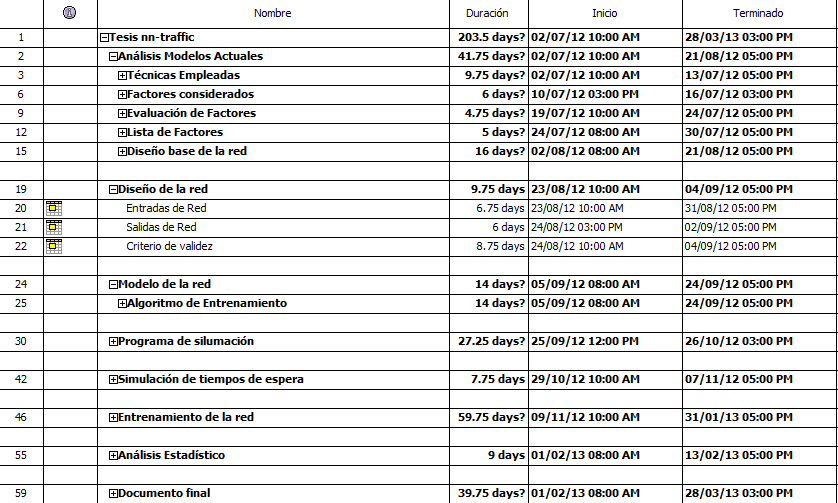
\includegraphics[width=1.1\textwidth,
 		height=0.65\textheight]{images/cronoMIN.png}
 		\caption{Cronograma}
 		\label{fig:Crono}
 	\end{figure}
	
	\begin{landscape}
	\begin{figure}[htp]
 		\centering 		
 		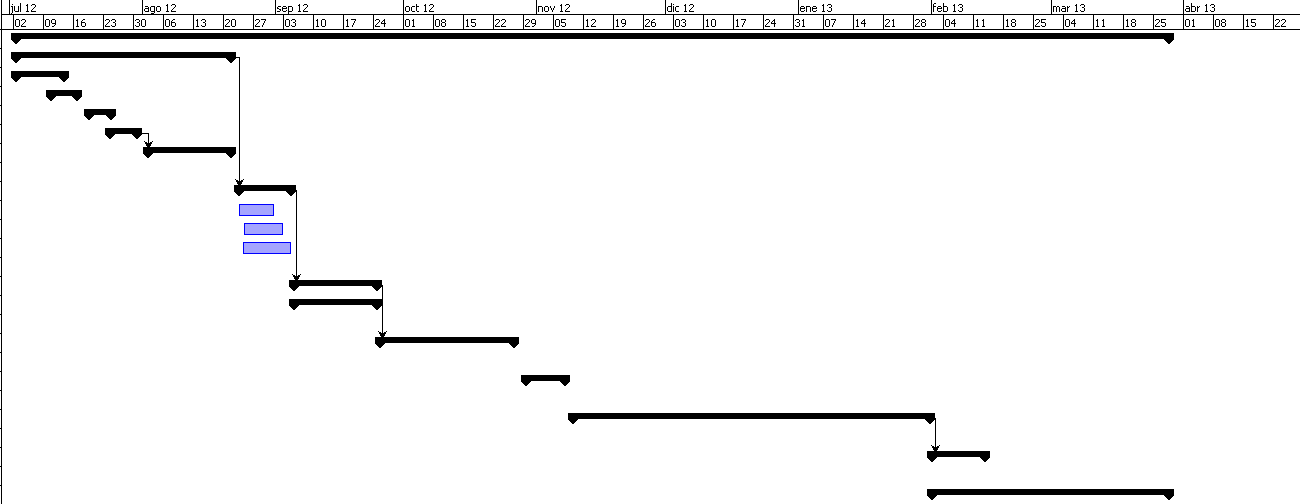
\includegraphics[width=20cm,height=15cm]{images/ganttMIN2.png}
 		\caption{Diagrama de Gantt}
 		\label{fig:gantt}
 	\end{figure}
	\end{landscape}
	
	\sectionbreak

% Final pages
\backmatter
\singlespace
%\bibliographystyle{apa}
\refstepcounter{chapter}

%\addcontentsline{toc}{chapter}{\bibname}
%\bibliography{body/references}
\chapter{Bibliograf\'{i}a}
	\label{chap:bib}
	
\begin{itemize}
  \item \textbf\textbf{[1]} Dobles R., (2011) Consecuencias de la contaminaci�n del aire
  y de la atm�sfera del sector energ�tico y tendencias de las emisiones contaminantes.
  Recupeardo de
  \url{http://www.amcham.co.cr/newsletters/201102/airecontamina.pdf}
  \item \textbf{[2]} Coxworth, B. (Septiembre, 2010) Self-regulating traffic lights would
  improve vehicle flow. Gizmag. Recuperado de
  \url{http://www.gizmag.com/self-regulating-traffic-lights-improve-vehicle-flow/16396/}
  \item \textbf{[3]} Gilmore J., Elibiary, K. (1993) Traffic Management Applications of
  Neural Networks. Recuperado de
  \url{http://www.aaai.org/Papers/Workshops/1993/WS-93-04/WS93-04-012.pdf}
  \item \textbf{[4]} Pramod K, Dongun S., Chima A. (2008) Automatic Traffic Light Control
  System. Recuperado desde \url{http://bit.ly/JMcl5R}
  \item \textbf{[5]}Centro de Control de Tr�fico MOPT (2011) Datos obtenidos del sistema.
  \item \textbf{[6]} Kriesel, D. (2005) A Brief Introduction to Neural Networks.
  Recuperado del sitio \url{http://www.dkriesel.com/en/science/neural_networks}
  \item \textbf{[7]} Hopfield, J (1962, Enero) Neural Networks and physical systems with
  emergent collective computational abilities. Pasadena, California
  \item Ayad M., M.S. Ahmad, M.Z.M. Yusoff, Hammad B. (s,f) Using Genetic
  Algorithm for Traffic Light Control System with a Pedestrian Crossing
  recuperado de: \url{http://paper.ijcsns.org/07_book/200902/20090212.pdf}
  \item \textbf{[9]} Rajendra Akerkar (2005) Introduction to Artificial Intelligence.
  Prentice-Hall OF India Private Limited, New Delhi. Pag 1-4
  \item \textbf{[10]} Greenman C., (1998) Choreographing the Dance of Traffic Lights. New
  York Times. Recuperado de http://www.nytimes.com/1998/09/17/technology/choreographing-the-dance-of-traffic-lights.html
  \item \textbf{[11]} Kumar G., (2007) Artificial Neural Network and Its Application. New
  Delhi. P�gs 2, 4 recuperado desde
  http://www.iasri.res.in/ebook/EBADAT/5-Modeling%20and%20Forecasting%20Techniques%20in%20Agriculture/5-ANN_GKJHA_2007.pdf
  \item \textbf{[12]} Gallant S., (1993) Neural Network Learning and Expert Systems. MIT
  Press. Pags 133
  \item \textbf{[14]} Loaiza V., (Noviembre, 2007) Capital estrena sem�foros inteligentes
  en 180 intersecciones. La Naci�n. Recuperado de
  \url{http://wvw.nacion.com/ln_ee/2007/noviembre/28/pais1332560.html}
  \item \textbf{[15]} Mata A., (Junio,2009) Acceso libre a San Jos� provoca colapso vial.
  La Naci�n, Costa Rica. Recuperado de
  \url{http://wvw.nacion.com/ln_ee/2009/junio/16/pais1997637.html}
  \item \textbf{[16]} Organisation for Economic Co-operation and Development, European
  Conference of Ministers of Transport, OECD/ECMT Transport Research Centre
  (2006) Speed Management. Recuperado de \url{http://bit.ly/KZjVZ9}
  \item \textbf{[17]} Fallas H., (2007) Choferes ven m�s presas en capital. La Naci�n.
  Recuperado de \url{http://wvw.nacion.com/ln_ee/2007/enero/29/pais976503.html}
  \item \textbf{[18]} Jameson et al Longo, Kasper. Harrison's Principles of internal
  medicine. McGraw Hill, 2011. URL
  \url{http://www.amazon.com/Harrisons-Principles-Internal-Medicine-Volumes/dp/007174889X/ref=sr_1_1?ie=UTF8&qid=1329942776&sr=8-1}
  \item \textbf{[19]} Hilera y Mart�nez. (1995) Redes Neuronales Artificiales.
  Fundamentos, Modelos y Aplicaciones. Addison Wesley
  \item \textbf{[20]} Graupe D., (2007) Principles of Artificial Neural Networks. World
  Scientific. Singapur
  \item \textbf{[21]} Dayan p., (s,f)  Unsupervised Learning. MIT. URL:
  \url{http://www.gatsby.ucl.ac.uk/~dayan/papers/dun99b.pdf}
  \item \textbf{[22]} Basogain X., (s,f) Redes Neuronales Artificiales y sus
  Aplicaciones. Espa�a. Url:
  \url{http://ocw.ehu.es/ensenanzas-tecnicas/redes-neuronales-artificiales-y-sus-aplicaciones/contenidos/pdf/libro-del-curso}
  \item \textbf{[23]} Srinivasan D., Chee M. et Long R., (2006) Neural Networks for
  RealTime Traffic Signal Control. IEEE. Singapur   Url:
  \url{http://www.jhuapl.edu/spsa/PDF-SPSA/Srinivasan_etal_IEEETITS06.pdf}
  \item \textbf{[24]} Ram�rez E., (2012) Reconocimiento de patrones en juegos utilizando
  redes neuronales. Tecnol�gico de Costa Rica.
  \item \textbf{[25]} Fritsch. Modular neural networks for speech recognition, 1996. URL
  \url{http://www.
dtic.mil/cgi-bin/GetTRDoc?AD=ADA326090&Location=U2&doc=GetTRDoc.pdf}
  
  \item \textbf{[26]} Brinckerhoff P., Farradyne T., (2010, Abril) Evaluation of Active
  Traffic Management Strategies. Recuperado de
  \url{http://www.metrocouncil.org/planning/transportation/MHSIS/AppEATMmodel.pdf}
  \item \textbf{[27]} Ezeel S., (2010, Enero)  Explaning International IT Application
  Leadership: Intelligent Transportation Systems. The Information Technology \& Innovation Foundation. Url:
  \url{http://www.itif.org/files/2010-1-27-ITS_Leadership.pdf}
  \item \textbf{[28]} Turnbull K, (s,f) Transit benefits from advanced transportation
  management centers. Texas Transportation Institute, USA URL:
  \url{http://www.etcproceedings.org/paper/transit-benefits-from-advanced-transportation-management-centres-45}
  \item \textbf{[29]} \url{http://ntl.bts.gov/lib/jpodocs/edldocs1/13480/ch3.pdf}
 
\end{itemize}

% \printglossaries
% \newglossaryentry{Neuronal network}{
% 	name = neuronalnet
% 	description={son modelos que intentan reproducir el comportamiento del cerebro
% 	humano.
% 	}
% }
\chapter{Glosario de T\'{e}rminos}
	\label{chap:term}
	
\begin{itemize}
  \item Actuated Operation: consiste de controladores de tr\'{a}fico y sensores de
  veh\'{i}culos localizados en las v\'{i}as que conducen a las intersecciones donde se han instalado los sem\'{a}foros y se ajustan los tiempos seg\'{u}n reglas.
  \item Algoritmo de Backpropagation: es un m\'{e}todo de aprendizaje
  supervisado empleado en el entrenamiento de redes neuronales que consta de dos fases.
  \item Ax\'{o}n: Extensi\'{o}n del soma con forma tubular y que tiende a ramificarse en
  uno de sus extremos.  
  \item Dendritas: ramificaciones localizadas en la parte superior de una
  neurona.  
  \item Pretimed Operation: forma de operaci\'{o}n en la cual las luces roja,
  amarilla y verde son temporizadas en intervalos fijos. 
  \item Red Neuronal: son modelos que intentan reproducir el comportamiento
  del cerebro humano.    
  \item Sistema Experto: sistema que cuenta con una base de conocimiento que se
  encuentra separada del sistema original, permitiendo agregar nuevo conocimiento a este sin requerirse realizar cambios al sistema.
  \item Soma: el n\'{u}cleo de una neurona biol\'{o}gica.
\end{itemize}


\end{document}
